% !TEX root = ../main.tex
\section{Classless D\&D} \label{sec::classlessdnd}
\DndDropCapLine{A}{n inch away from death, a band of}
fellows barely manages to escape from a bloodthirsty nidhogg.
Worn and weary, they settle against an outcrop of rocks, taking a moment to catch their breath.

Nightfall comes all too fast, and they improvise a campfire to keep them warm during the night.
Just as they begin their well-deserved rest, they feel an unsettling rumbling beneath their feet.
What they originally thought was a strange-looking rock starts moving, revealing itself to be a troll.
Tired they scramble for arms, a gat grabbing their mace, and an ird her trusty quarterstaff.

\subsection*{Call to Adventure}
    Adventurers leave home as any person would, picking up an assortment of skills and feats on the road.
    Unskilled and untrained, they take their time to become experts in what they do.
    Lest they become prey to a savage beast or an opportunist bandit.

\subsection*{Creating a character}
    Your first step in playing is creating a character of your own.
    You choose a kin, which will determine their physical characteristics and provide them with a set of traits.
    Then, you choose a background, which describes what they did before joining the adventuring life and provides them with one feature.
    Additionally, your character's kin and background will give them access to a specific set of feats.
    You also choose your character's tidal alignment, invent the personality, appearance, and backstory of your character.

    \subsubsection{Ability Scores}
        After choosing your character's kin and background, it's time to generate their ability scores randomly.
        Roll four d6s and record the total of the highest three dice on a piece of scratch paper.
        Do this five more times, so that you have six numbers.

        Now take your six numbers and write each beside one of your character's six abilities to assign scores to Strength, Dexterity, Constitution, Intelligence, Wisdom, and Charisma.
        Afterward, make any changes to your ability scores as a result of your kin choice.

        After assigning your ability scores, determine your ability modifiers.
        This is done by subtracting 10 from the ability score and then dividing the result by 2 (round down).
        Write the modifier next to each of your scores.

    \subsubsection{Hit Points and Hit Dice}
        On creation, your character has a number of hit points equal to 8 + their Constitution modifier.
        Upon leveling up, roll a d8 and add the number rolled + your character's Constitution modifier to their hit point pool.
        Alternatively, you can forgo this roll and simply add 5 + your character's Constitution modifier.

        Your character has a number of hit dice equal to their level.
        By default all these hit dice are d8s, but they can be improved (or worsened) by taking relevant major character advancement, which are described in their own section at page \pageref{ssec::majorcharacteradvancement}.

    \subsubsection{Proficiency Levels}
        Instead of having one particular proficiency bonus, your character has specific proficiency levels in different skills, proficiencies, and saving throws.
        Proficiency levels in skills and proficiencies are gained via feats, while in saving throws they are gained at specific levels, as is listed in the Character Progression Table.

        There are five proficiency levels:
        \subparagraph{Untrained} Completely unskilled in the practice, you have no proficiency bonus.
        \subparagraph{Competent} Some basic experience gives you a +2 proficiency bonus.
        \subparagraph{Skilled} Practice makes perfect, you have a +4 proficiency bonus.
        \subparagraph{Expert} A fully realized professional, you have a +6 proficiency bonus.
        \subparagraph{Legendary} Your skill is lauded, and your crafts acclaimed.
        You have a +12 proficiency bonus.

    % NOTE: It might be cool to find a way to make this look more like the official class summary tables.
    \begin{DndTable}[width=\linewidth, header=Character Progression Table]{ccl}
        \textbf{Level} & \textbf{Required FP} & \textbf{Feature} \\
        1              & 0                    & 2 Saving Throw Improvements \\
        2              & 1                    & Ability Score Improvement \\
        3              & 2                    & Major Character Advancement \\
        4              & 3                    & Ability Score Improvement \\
        5              & 5                    & Saving Throw Improvement \\
        6              & 7                    & Ability Score Improvement \\
        7              & 9                    & - \\
        8              & 11                   & Ability Score Improvement \\
        9              & 13                   & Saving Throw Improvement \\
        10             & 15                   & Ability Score Improvement \\
        11             & 18                   & Major Character Advancement \\
        12             & 21                   & Ability Score Improvement \\
        13             & 24                   & Saving Throw Improvement \\
        14             & 27                   & Ability Score Improvement \\
        15             & 30                   & - \\
        16             & 34                   & Ability Score Improvement \\
        17             & 39                   & Saving Throw Improvement \\
        18             & 44                   & Ability Score Improvement \\
        19             & 51                   & Major Character Advancement \\
        20             & 60                   & Ability Score Improvement
    \end{DndTable}

% !TEX root = ../main.tex
\subsection*{Beyond First Level} \label{ssec::beyondfirstlevel}
\DndDropCapLine{W}{ith one heavy loss, the group}
dispatches the fearsome troll.
They perform a small funerary ritual, to then finally get some rest.
Beaten and tired, they learned their lesson for the day.

\thispagestyle{empty}
\begin{tikzpicture}[remember picture,overlay]
    \node[anchor=south, yshift=-0.10cm] at (current page.south) {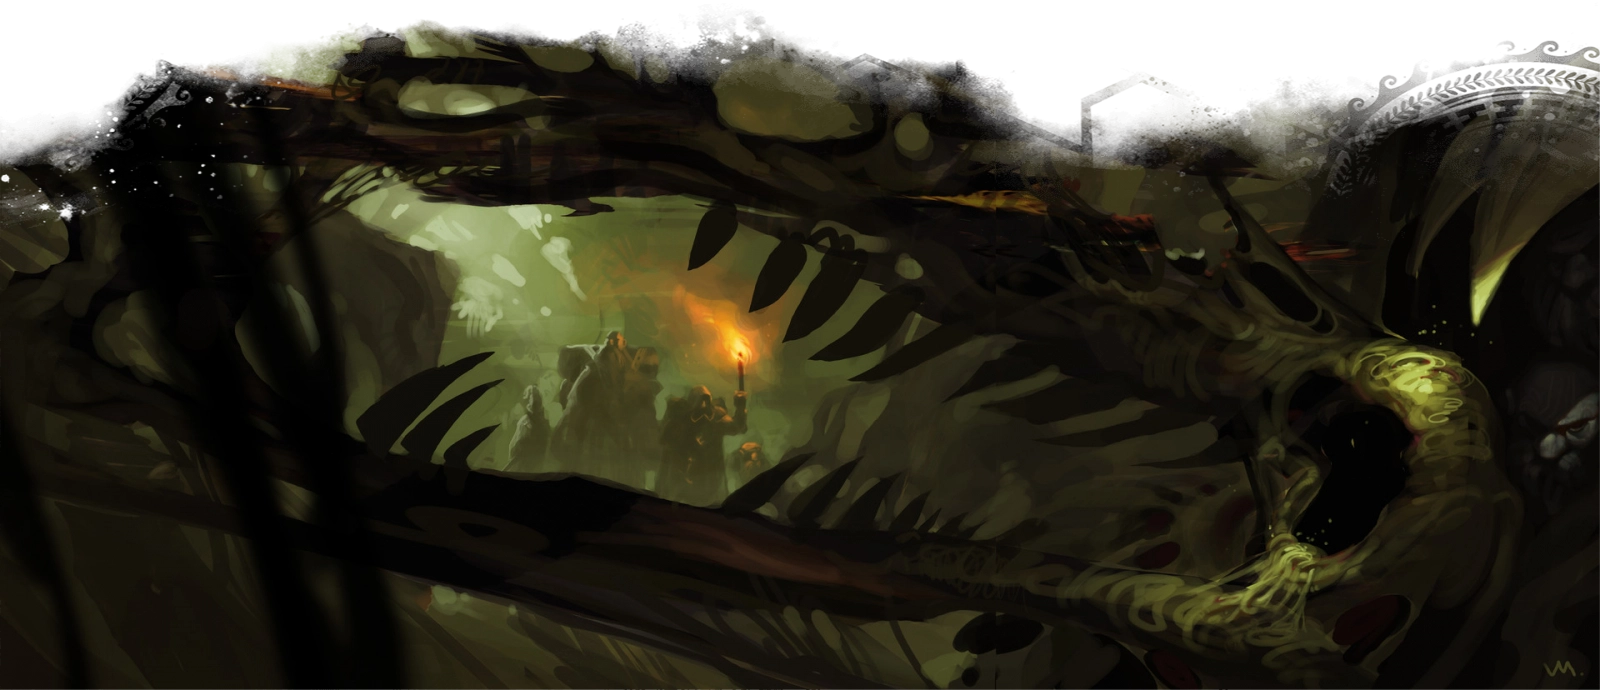
\includegraphics[width=\pdfpagewidth]{03mechanics/img/21jungle_adventure}};
\end{tikzpicture}

\subsubsection{Experience}
    What is learned by your character during the game is measured by Experience Points (XP).
    After you finish playing, talk about the session with the whole group and discuss what happened.
    Read the questions in the table below.
    For each of them that you can reply ``yes'' to, your character gets one XP.

    \begin{itemize}
        \item Did you participate in the session?
        \item Did you travel to a new location?
        \item Did you defeat one or more creatures?
        \item Did you loot treasure?
        \item Did you complete a quest?
        \item Did you solve a conflict?
        \item Did you make a new friend, ally, or enemy?
        \item Did you help another PC?
        \item Did your ideals, bonds, or flaws affect any of your decisions during the session?
        \item Did you perform any action related to your kin, background, or origin?
        \item Did you perform an extraordinary action of some kind?
    \end{itemize}

    In case of any discussion or disagreement, the DM always has the last word.
    Additional XP may be awarded when specific story milestones are achieved, but this too is left to the discretion of the DM.

    \newpage

\subsubsection{Feat Points}
    As your character adventures, they will gain \textbf{Feat Points} (FP).
    Feat points are spent to buy feats, which can only be done as part of a long rest.
    You can buy multiple feats in one long rest.
    Feats either increase your proficiency level at a skill or a proficiency, or they include a useful feature.

    When you reach 10 XP, reset your XP counter and add one FP, keeping the remaining XP.
    Feat points are used to learn new feats, which include either an increase in a proficiency level or a feature.

    You don't need to spend FP right after earning it, you can save as many as you want for as long as you need.
    The full list of feats starts in the next page.

    A new character has a number of FP equal to 3 plus the number of FP that would be required to reach the character's level if it had leveled normally.

\subsubsection{Leveling Up}
    As your character gains feat points they will gain levels, acquiring hit dice, improving their ability scores and saving throw proficiencies, and gaining major character advancements.
    \begin{itemize}
        \item Ability Score Improvements allow you to increase one of you ability scores by 1 up to a maximum of 20.
        \item Saving Throw Improvements increase your level of proficiency on a saving throw of your choice by one, to a maximum of Expert proficiency.
        \item Major Character Advancements are character-defining improvements which include hit dice upgrades, combat styles, and proficiency improvements.
        They are listed in page \pageref{ssec::majorcharacteradvancement}.
    \end{itemize}

    When your Constitution modifier increases by 1 or you improve your hit dice, your hit point maximum increases by 1 for each level you have attained.
    Similarly, you decrease your hit point maximum by 1 if you worsen your hit dice.

    \newpage

% !TEX root = ../main.tex
\addcontentsline{toc}{section}{Feats}
\subsection*{Feats} \label{ssec::feats}
For simplicity, feats are separated into six categories: feats related to kin, background, skills, proficiencies, combat, and spellcasting.
Kin, background, proficiencies, and spellcasting feats are detailed in their corresponding chapters, while skills and combat feats are described in this section.
In addition, lists with all the feats are contained in the following pages.

Unless specified otherwise, a feat can only be learned once.

% !TEX root = ../main.tex
\addcontentsline{toc}{section}{Skill Feats}
\subsection*{Skill Feats}
\begin{DndTable}[width=\linewidth, header=Skill Feat List 1/3]{ll}
    \textbf{Ability Score or Skill} & \textbf{Feat}                                               \\
    Strength & \textbf{Brute} (page \pageref{feat::brute})                                        \\
    Strength & \textbf{Chair Juggler} (page \pageref{feat::chairjuggler})                         \\
    Strength & \textbf{Feeble} (page \pageref{feat::feeble})                                      \\
    Strength & \textbf{Powerful Build} (page \pageref{feat::powerfulbuild_skill})                 \\
    Strength & \textbf{Powerhouse} (page \pageref{feat::powerhouse})                              \\

    Dexterity & \textbf{Clumsy Reflex} (page \pageref{feat::clumsyreflex}                         \\
    Dexterity & \textbf{Evasion} (page \pageref{feat::evasion}                                    \\
    Dexterity & \textbf{Nimble} (page \pageref{feat::nimble}                                      \\
    Dexterity & \textbf{Otherwordly Agility} (page \pageref{feat::otherwordlyagility}             \\
    Dexterity & \textbf{Quick Dodge} (page \pageref{feat::quickdodge}                             \\

    Constitution & \textbf{Brawny Defense} (page \pageref{feat::brawnydefense})                   \\
    Constitution & \textbf{Cling to Life} (page \pageref{feat::clingtolife})                      \\
    Constitution & \textbf{Hit Die Improvement} (page \pageref{feat::hitdieimprovement})          \\
    Constitution & \textbf{Pitiful} (page \pageref{feat::pitiful})                                \\
    Constitution & \textbf{Second Wind} (page \pageref{feat::secondwind})                         \\

    Intelligence & \textbf{Above and Beyond} (page \pageref{feat::aboveandbeyond})                \\
    Intelligence & \textbf{Knowledgeable Craft} (page \pageref{feat::knowledgeablecraft})         \\
    Intelligence & \textbf{Let Me Try!} (page \pageref{feat::letmetry})                           \\
    Intelligence & \textbf{Quick Wit} (page \pageref{feat::quickwit})                             \\
    Intelligence & \textbf{Smart Remark} (page \pageref{feat::smartremark})                       \\

    Wisdom & \textbf{Astute Defense} (page \pageref{feat::astutedefense})                         \\
    Wisdom & \textbf{Eye for the Opportunity} (page \pageref{feat::eyefortheopportunity})         \\
    Wisdom & \textbf{Insightful Fighter} (page \pageref{feat::insightfulfighter})                 \\
    Wisdom & \textbf{Unwise Decision} (page \pageref{feat::unwisedecision})                       \\
    Wisdom & \textbf{Wizened by Experience} (page \pageref{feat::wizenedbyexperience})            \\

    Charisma & \textbf{Anticharm} (page \pageref{feat::anticharm})                                \\
    Charisma & \textbf{Emboldening Visage} (page \pageref{feat::emboldeningvisage})               \\
    Charisma & \textbf{Enamoring Face} (page \pageref{feat::enamoringface})                       \\
    Charisma & \textbf{Force of Inspiration} (page \pageref{feat::forceofinspiration})            \\
    Charisma & \textbf{Saving Face} (page \pageref{feat::savingface})                             \\

    \textbf{Acrobatics} & \textbf{Acrobat} (page \pageref{feat::acrobat})                         \\
    Acrobatics & \textbf{Aerialist} (page \pageref{feat::aerialist})                              \\
    Acrobatics & \textbf{All-Terrain} (page \pageref{feat::allterrain})                           \\
    Acrobatics & \textbf{Fleet Footed} (page \pageref{feat::fleetfooted})                         \\
    Acrobatics & \textbf{Mobile} (page \pageref{feat::mobile})                                    \\

    \textbf{Animal Handling} & \textbf{Animal Handler} (page \pageref{feat::animalhandler})       \\
    Animal Handling & \textbf{Animal Companion} (page \pageref{feat::animalcompanion})            \\
    Animal Handling & \textbf{Sympathetic} (page \pageref{feat::sympathetic})                     \\
    Animal Handling & \textbf{Tamer} (page \pageref{feat::tamer})                                 \\
    Animal Handling & \textbf{Zoophilist} (page \pageref{feat::zoophilist})                       \\

    \textbf{Arcana} & \textbf{Arcanist} (page \pageref{feat::arcanist})                           \\
    Arcana & \textbf{Countercaster} (page \pageref{feat::countercaster})                          \\
    Arcana & \textbf{Gifted} (page \pageref{feat::gifted})                                        \\
    Arcana & \textbf{Identify} (page \pageref{feat::identify})                                    \\
    Arcana & \textbf{Metamagic Initiate} (page \pageref{feat::metamagicinitiate})                 %\\
\end{DndTable}
\begin{DndTable}[width=\linewidth, header=Skill Feat List 2/3]{ll}
    \textbf{Athletics} & \textbf{Athlete} (page \pageref{feat::athlete})                          \\
    Athletics & \textbf{Always Ready} (page \pageref{feat::alwaysready})                          \\
    Athletics & \textbf{Jogger} (page \pageref{feat::jogger})                                     \\
    Athletics & \textbf{Robust} (page \pageref{feat::robust})                                     \\
    Athletics & \textbf{Strong Body} (page \pageref{feat::strongbody})                            \\

    \textbf{Deception} & \textbf{Deceiver} (page \pageref{feat::deceiver})                        \\
    Deception & \textbf{Convincing Speech} (page \pageref{feat::convincingspeech})                \\
    Deception & \textbf{Feign Innocence} (page \pageref{feat::feigninnocence})                    \\
    Deception & \textbf{Liar} (page \pageref{feat::liar})                                         \\
    Deception & \textbf{Taunt} (page \pageref{feat::taunt})                                       \\

    \textbf{History} & \textbf{Historian} (page \pageref{feat::historian})                        \\
    History & \textbf{Advisor} (page \pageref{feat::advisor})                                     \\
    History & \textbf{Cognizant} (page \pageref{feat::cognizant})                                 \\
    History & \textbf{Sharpened Mind} (page \pageref{feat::sharpenedmind})                        \\
    History & \textbf{Wizened Advice} (page \pageref{feat::wizenedadvice})                        \\

    \textbf{Insight} & \textbf{Insightful} (page \pageref{feat::insightful})                      \\
    Insight & \textbf{Awesome Alertness} (page \pageref{feat::awesomealertness})                  \\
    Insight & \textbf{Incredible Intuition} (page \pageref{feat::incredibleintuition})            \\
    Insight & \textbf{Keen Mind} (page \pageref{feat::keenmind})                                  \\
    Insight & \textbf{Uncanny Insight} (page \pageref{feat::uncannyinsight})                      \\

    \textbf{Intimidation} & \textbf{Intimidating} (page \pageref{feat::intimidating})             \\
    Intimidation & \textbf{Demoralize} (page \pageref{feat::demoralize})                          \\
    Intimidation & \textbf{Frightful Presence} (page \pageref{feat::frightfulpresence})           \\
    Intimidation & \textbf{Inspire Fear} (page \pageref{feat::inspirefear})                       \\
    Intimidation & \textbf{Menacing} (page \pageref{feat::menacing})                              \\

    \textbf{Investigation} & \textbf{Investigative} (page \pageref{feat::investigative})          \\
    Investigation & \textbf{Detective} (page \pageref{feat::detective})                           \\
    Investigation & \textbf{Eye for Weakness} (page \pageref{feat::eyeforweakness})               \\
    Investigation & \textbf{Inquisitive} (page \pageref{feat::inquisitive})                       \\
    Investigation & \textbf{Unerring Eye} (page \pageref{feat::unerringeye})                      \\

    \textbf{Medicine} & \textbf{Medic} (page \pageref{feat::medic})                               \\
    Medicine & \textbf{Guardian Angel} (page \pageref{feat::guardianangel})                       \\
    Medicine & \textbf{Healer's Insight} (page \pageref{feat::healersinsight})                    \\
    Medicine & \textbf{Refined Healing} (page \pageref{feat::refinedhealing})                     \\
    Medicine & \textbf{Restoring Rest} (page \pageref{feat::restoringrest})                       \\

    \textbf{Nature} & \textbf{Naturalist} (page \pageref{feat::naturalist})                       \\
    Nature & \textbf{Deft Explorer} (page \pageref{feat::deftexplorer})                           \\
    Nature & \textbf{Experienced Traveler} (page \pageref{feat::experiencedtraveler})             \\
    Nature & \textbf{Hide in Plain Sight} (page \pageref{feat::hideinplainsight})                 \\
    Nature & \textbf{Natural Awareness} (page \pageref{feat::naturalawareness})                   \\

    \textbf{Perception} & \textbf{Perceptive} (page \pageref{feat::perceptive})                   \\
    Perception & \textbf{Blindsense} (page \pageref{feat::blindsense})                            \\
    Perception & \textbf{Hawk-eyed} (page \pageref{feat::hawkeyed})                               \\
    Perception & \textbf{Refined Sight} (page \pageref{feat::refinedsight})                       \\
    Perception & \textbf{Reliable Sight} (page \pageref{feat::reliablesight})                     \\

    \textbf{Performance} & \textbf{Performer} (page \pageref{feat::performer})                    \\
    Performance & \textbf{Actor} (page \pageref{feat::actor})                                     \\
    Performance & \textbf{Enthralling Performance} (page \pageref{feat::enthrallingperformance})  \\
    Performance & \textbf{Flourished Duelist} (page \pageref{feat::flourishedduelist})            \\
    Performance & \textbf{Soothing Presence} (page \pageref{feat::soothingpresence})              \\

    \textbf{Persuasion} & \textbf{Persuasive} (page \pageref{feat::persuasive})                   \\
    Persuasion & \textbf{Eloquent} (page \pageref{feat::eloquent})                                \\
    Persuasion & \textbf{Haggler} (page \pageref{feat::haggler})                                  \\
    Persuasion & \textbf{Reliever} (page \pageref{feat::reliever})                                \\
    Persuasion & \textbf{Therapist} (page \pageref{feat::therapist})                              \\

    \textbf{Religion} & \textbf{Theologian} (page \pageref{feat::theologian})                     \\
    Religion & \textbf{Holy Fortitude} (page \pageref{feat::holyfortitude})                       \\
    Religion & \textbf{Peace of Mind} (page \pageref{feat::peaceofmind})                          \\
    Religion & \textbf{Pious} (page \pageref{feat::pious})                                        \\
    Religion & \textbf{Student of the Tides} (page \pageref{feat::studentofthetides})             \\

    \textbf{Sleight of Hand} & \textbf{Quick Fingers} (page \pageref{feat::quickfingers})         \\
    Sleight of Hand & \textbf{Fast Hands} (page \pageref{feat::fasthands})                        %\\
\end{DndTable}
\begin{DndTable}[width=\linewidth, header=Skill Feat List 3/3]{ll}
    Sleight of Hand & \textbf{Phantom} (page \pageref{feat::phantom})                             \\
    Sleight of Hand & \textbf{Pickpocket} (page \pageref{feat::pickpocket})                       \\
    Sleight of Hand & \textbf{Poacher} (page \pageref{feat::poacher})                             \\

    \textbf{Stealth} & \textbf{Sneak} (page \pageref{feat::sneak})                                \\
    Stealth & \textbf{Ghost} (page \pageref{feat::ghost})                                         \\
    Stealth & \textbf{Hidden Striker} (page \pageref{feat::hiddenstriker})                        \\
    Stealth & \textbf{Skulker} (page \pageref{feat::skulker})                                     \\
    Stealth & \textbf{Sly} (page \pageref{feat::sly})                                             \\

    \textbf{Survival} & \textbf{Survivor} (page \pageref{feat::survivor})                         \\
    Survival & \textbf{Always on Track} (page \pageref{feat::alwaysontrack})                      \\
    Survival & \textbf{Hunter's Sense} (page \pageref{feat::hunterssense})                        \\
    Survival & \textbf{Trained by Nature} (page \pageref{feat::trainedbynature})                  \\
    Survival & \textbf{Tracker} (page \pageref{feat::tracker})                                    %\\
\end{DndTable}

% A
\subsubsection{Above and Beyond (2 FP)} \label{feat::aboveandbeyond}
    Your intelligence puts you above common mortals.
    Increase your proficiency with a skill or tool proficiency with which you are an Expert to Legendary, increasing your proficiency bonus with it to +12.
    \paragraph{Requirements} Intelligence 21. Expert proficiency in the relevant skill.
\subsubsection{Acrobat} \label{feat::acrobat}
    You increase your proficiency level in the Acrobatics skill.
    This feat can be taken three times, or until you reach Expert proficiency on the skill.
\subsubsection{Actor} \label{feat::actor}
    A natural performer, you've never failed to impress with your refined acting skills.
    % You have an easy time imitating the demeanor of others, especially of those that you know well.
    You can take this feat three times, gaining different effects each time:
    \begin{itemize}
        \item You have advantage on ability checks trying to pass off as another member of your kin, even without a disguise.
        \item You have advantage on Charisma (Deception) and Charisma (Performance) checks when trying to pass yourself off as a different person of any kin.
        If you are wearing a good quality outfit, you can pass these checks automatically.
        \item You can mimic the speech of another person or the sounds made by other creatures.
        You must have heard the person speaking, or heard the creature make the sound, for at least 1 minute.
        A successful Wisdom (Insight) check contested by your Charisma (Deception) or Charisma (Performance) check allows a listener to determine that the effect is faked.
    \end{itemize}
    \paragraph{Requirements} Skilled proficiency in the Performance skill.
\subsubsection{Advisor (2 FP)} \label{feat::advisor}
    As an action, you can give a creature a bonus equal to your proficiency bonus with the History skill to any ability check or saving throw.
    The creature must be able to hear and understand you.

    You can use this ability a number of times equal to your Intelligence modifier (Minimum of one).
    \paragraph{Requirements} Expert proficiency in the History skill.
\subsubsection{Aerialist} \label{feat::aerialist}
    You've had an exceptional flexibility from a very young age.
    You can make a running long jump or a running high jump after moving only 1 meter or foot, rather than 2 meters.
    \paragraph{Requirements} Competent proficiency in the Acrobatics skill.
\subsubsection{All-Terrain} \label{feat::allterrain}
    Moving through difficult terrain costs you no extra movement.
    \paragraph{Requirements} Skilled proficiency in the Acrobatics skill.
\subsubsection{Always on Track} \label{feat::alwaysontrack}
    You make Wisdom (Survival) ability checks to find your way with advantage.
    % and your group can't become lost except by magical means.
    \paragraph{Requirements} Competent proficiency in the Survival skill.
\subsubsection{Always Ready} \label{feat::alwaysready}
    Your physical prowess is a marvel to most.
    When you are prone, standing up doesn't provoke attacks of opportunity.
    \paragraph{Requirements} Competent proficiency in the Athletics skill.
\subsubsection{Animal Companion (2 FP)} \label{feat::animalcompanion}
    You can try to bond with a wild creature that is not violent towards you and has a number of hit dice equal or lower than yours.
    Make a Wisdom (Animal Handling) check contested by the creature's Wisdom (Insight).
    The creature's roll gains a bonus equal to half its number of hit dice (rounded down).
    If you succeed, you can spend 8 hours bonding with the beast, after which it becomes your animal companion.

    The beast rolls initiative as normal and acts on its own volition during its turns.
    On its turns, it will defend itself and you against aggressors.
    You can issue commands to it as an action without needing to make an ability check, and when you do so you can control the beast during its next turn.
    It never requires your command to use its reaction, such as when making an opportunity attack.

    If you are incapacitated or absent, your beast companion will act on its own, focusing on protecting you and itself.

    If you fail on the check, you fail to bond and you cannot try to bond with the same beast again.
    \paragraph{Requirements} Expert proficiency in the Animal Handling skill.
\subsubsection{Animal Handler} \label{feat::animalhandler}
    You increase your proficiency level in the Animal Handling skill.
    This feat can be taken three times, or until you reach Expert proficiency on the skill.
\subsubsection{Anticharm} \label{feat::anticharm}
    As an action, you can try to charm a creature.
    The creature must roll a Wisdom saving throw with a DC equal to 12 + your Charisma modifier.
    On a success, you disgust the creature so much that it has disadvantage on attack rolls against creatures other than you, and you have disadvantage on any ability check to interact socially with it.
    This effect lasts until the end of your next turn.
    On a failure, nothing happens.

    If your Charisma score increases above 9 through any means you lose the benefits of this feat.
    You can only regain them by lowering your Charisma score back to 9 or lower.
    \paragraph{Requirements} Wisdom of 9 or lower.
\subsubsection{Arcanist} \label{feat::arcanist}
    You increase your proficiency level in the Arcana skill.
    This feat can be taken three times, or until you reach Expert proficiency on the skill.
\subsubsection{Astute Defense} \label{feat::astutedefense}
    If you are unarmored, your AC equals your Dexterity ability modifier + your Wisdom ability modifier.
    \paragraph{Requirements} Wisdom 15.
\subsubsection{Athlete} \label{feat::athlete}
    You increase your proficiency level in the Athletics skill.
    This feat can be taken three times, or until you reach Expert proficiency on the skill.
\subsubsection{Awesome Alertness (2 FP)} \label{feat::awesomealertness}
    You are permanently aware of danger, and have advantage on initiative rolls.

    In addition, you and any of your companions within 6 meters of you can't be surprised, except when incapacitated by something other than nonmagical sleep.
    You instantly awaken if you are sleeping naturally when combat begins.
    \paragraph{Requirements} Expert proficiency in the Insight skill.
% B
\subsubsection{Blindsense (2 FP)} \label{feat::blindsense}
    Unnaturally perceptive, you gain tremorsense with a radius of 2 meters and blindsight with a radius of 6 meters.
    Tremorsense allows you to perceive anything on the ground or below, while blindsight allows you to perceive your surroundings without reyling on sight.
    \paragraph{Requirements} Expert proficiency in the Perception skill.
\subsubsection{Brawny Defense} \label{feat::brawnydefense}
    If you are unarmored, your AC equals your Dexterity ability modifier + your Constitution ability modifier.
    \paragraph{Requirements} Constitution 15.
\subsubsection{Brute} \label{feat::brute}
    You can take the Overrun action (see page \pageref{act::overrun}) as part of your movement.
    \paragraph{Requirements} Strength 12.
% C
\subsubsection{Cling to Life (2 FP)} \label{feat::clingtolife}
    Resilient even in the face of death, you roll death saving throws with advantage.

    In addition, if you are attacked while unconscious, you can roll a Constitution saving throw with a DC equal to 10 or half the damage done, whichever's higher.
    If you succeed, you don't suffer a death saving throw failure.
    \paragraph{Requirements} Constitution 21.
\subsubsection{Clumsy Reflex} \label{feat::clumsyreflex}
    You use your clumsiness to your advantage, and can use your reaction to gain advantage on a Dexterity saving throw.
    As you flail about, any creature (friend or foe) within 1 meter of you that makes a Dexterity saving throw does so with disadvantage.

    You can use this ability two times, and you regain all expended uses on a short rest.

    If your Dexterity score increases above 9 through any means you lose the benefits of this feat.
    You can only regain them by lowering your Dexterity score back to 9 or lower.
    \paragraph{Requirements} Dexterity of 9 or lower.
\subsubsection{Cognizant} \label{feat::cognizant}
    From background or perchance you've been given a privileged access to books and teaching thorough your life.
    You have advantage on Intelligence (History) checks to recall any information of your kin and your country of origin.
    \paragraph{Requirements} Competent proficiency in the History skill.
\subsubsection{Convincing Speech} \label{feat::convincingspeech}
    You can take this feat three times, gaining different effects each time:
    \begin{itemize}
        \item You don't gain disadvantage on Charisma (Deception) or Charisma (Persuasion) checks made in the middle of combat.
        \item Using two actions, you can attempt to deceive one person you can see within 6 meters of you who can see and hear you.
        Make a Charisma (Deception) check contested by the target's Wisdom (Insight) check.
        If your check succeeds, your movement doesn't provoke opportunity attacks from the target and your attack rolls against it have advantage; both benefits last until the end of your next turn or until you use this ability on a different target.
        If your check fails, the target can't be deceived by you in this way for one hour.
        \item If nor you or your allies attack the deceived person, it becomes convinced that you are their allies and will stop attacking you and your companions for a minute.
        The creature rolls a Wisdom saving throw with a DC equal to the number you rolled in your Charisma (Deception) check at the end of its turns.
        Its allies can help it so that it makes this roll with advantage.
        The target can't be deceived by you in this way for 1 hour after winning or failing the contest.
    \end{itemize}
    \paragraph{Requirements} Skilled proficiency in the Deception skill.
\subsubsection{Countercaster (2 FP)} \label{feat::countercaster}
    Educated in all sorts of doctrines, you have advantage in the Identify a Spell action.
    In addition, when you identify a spell you can try to prevent it from being casted.
    If the casting creature is no more than 12 meters away from you, you can roll another Intelligence (Arcana) check with a DC equal to 15 + the spell's level using the same reaction.
    On a success, the creature's spell fails and has no effect.
    \paragraph{Requirements} Expert proficiency in the Arcana skill.
% D
\subsubsection{Deceiver} \label{feat::deceiver}
    You increase your proficiency level in the Deception skill.
    This feat can be taken three times, or until you reach Expert proficiency on the skill.
\subsubsection{Deft Explorer} \label{feat::deftexplorer}
    Your appreciation for nature has led you to attain an extensive categorical knowledge of plants and animals, giving you a great feat at recognizing and identifying them.

    Provided you are familiar with the local flora and fauna from experience or a guide, you don't need to make an ability check to identify common plants, fungi, animals, and insects.
    You gain familiarity with a region by taking a long rest in it.
    \paragraph{Requirements} Competent proficiency in the Nature skill.
\subsubsection{Demoralize} \label{feat::demoralize}
    You can use two actions to attempt to demoralize one creature within 6 meters of you that can see and hear you.
    Make a Charisma (Intimidation) check contested by the target's Wisdom (Insight) check.
    If you succeed, the target is frightened of you for a minute.
    In addition, it makes all attack rolls with disadvantage for that duration.
    The creature can make a Wisdom saving throw at the end of its turns with a DC equal to the number you rolled to end this effect.

    If you fail, the target can't be frightened by you in this way for one hour.
    \paragraph{Requirements} Skilled proficiency in the Intimidation skill.
\subsubsection{Detective} \label{feat::detective}
    You reduce the action cost of the Search action to one action.
    \paragraph{Requirements} Skilled proficiency in the Investigation skill.
% E
\subsubsection{Eloquent} \label{feat::eloquent}
    A skilled negotiator and a master of diplomacy, you have an easy time convincing people to do what you need.
    You can take this feat three times, gaining different benefits each time:
    \begin{itemize}
        \item You gain advantage on Charisma (Persuasion) ability checks and contests made against creatures that do not see you as a threat or an enemy in any way.
        \item If you spend one minute talking to someone who can understand what you say, you can make a Charisma (Persuasion) check contested by the creature's Wisdom (Insight).
        If you or your companions are fighting the creature, the check automatically fails.
        If you succeed, the target is charmed by you as long as it remains within 12 meters of you and for 5 minutes thereafter.
        If you or your companions attack the creature, the charm ends.
        \item Your otherwordly charisma is hard to forget.
        Any creature that you have charmed in the past remembers you and can offer you favors as long as they're reasonable.
    \end{itemize}
    \paragraph{Requirements} Skilled proficiency in the Persuasion skill.
\subsubsection{Emboldening Visage} \label{feat::emboldeningvisage}
    All friendly creatures (excluding yourself) that are within 3 meters of you gain a bonus to all saving throws equal to half your Charisma modifier (rounded down).
    \paragraph{Requirements} Charisma 18.
\subsubsection{Enamoring Face (2 FP)} \label{feat::enamoringface}
    When any creature forces you to roll a saving throw or become charmed, you can counter-charm them as a reaction, even if you fail the saving throw.
    The creature must roll a Wisdom saving throw with a DC equal to 10 + your Charisma modifier.
    Upon failure, the creatured is charmed by you for a minute or until you do anything harmful to it.
    \paragraph{Requirements} Charisma 21.
\subsubsection{Enthralling Performance (2 FP)} \label{feat::enthrallingperformance}
    While performing, you can try to distract anyone who can see and hear you.
    Make a Charisma (Performance) check contested by the each person's Wisdom (Insight) check.
    If you check succeeds, you grab the person's attention enough that it automatically fails on Wisdom (Perception) and Intelligence (Investigation).
    You can tell which people have failed and succeeded on the contest.

    Any person enthralled by your performance will remember it for a lifetime.
    They will remember you and can offer you favors as long as they are reasonable.
    \paragraph{Requirements} Expert proficiency in the Performance skill.
\subsubsection{Evasion} \label{feat::evasion}
    You can nimbly dodge out of the way of certain area effects, such as a wyvern's acid breath or an ice storm spell.
    When you are subjected to an effect that allows you to make a Dexterity saving throw to take only half damage, you instead take no damage if you succeed on the saving throw, and only half damage if you fail.
    \paragraph{Requirements} Dexterity 18.
\subsubsection{Experienced Traveler} \label{feat::experiencedtraveler}
    You are an unsurpassed explorer, using your uncanny knowledge of nature to understand and survive in any environment.
    You can take this feat multiple times, obtaining different effects each time:
    \begin{itemize}
        \item Difficult Terrain doesn't slow your group's travel.
        \item When you forage, you find twice as much food as you normally would.
        \item While tracking down creatures, you also learn their exact number, their sizes, and how long ago they passed through the area.
    \end{itemize}
    \paragraph{Requirements} Skilled proficiency in the Nature skill.
\subsubsection{Eye for the Opportunity (2 FP)} \label{feat::eyefortheopportunity}
    Always attentive of your surroundings, you can use your reaction to make opportunity attacks against creatures when they enter your reach.
    In addition, you score critical hits with opportunity attacks on a roll of 19 or 20 on the d20.
    If you have the Improved Critical feat (see page \pageref{feat::improvedcritical}), this range is extended to rolls between 18 and 20 on the d20.
    Additionally, if you have that feat and the Superior Critical feat (see page \pageref{feat::superiorcritical}), this range is further extended to rolls between 17 and 20.
    \paragraph{Requirements} Wisdom 21.
\subsubsection{Eye for Weakness (2 FP)} \label{feat::eyeforweakness}
    You learn to exploit a creature's weaknesses by carefully studying its tactics and movement.
    You learn the \textbf{Aim} action (see page \pageref{act::aim}).
    When you successfully attack a creature after using this action, you roll the weapon's damage die one additional time.
    \paragraph{Requirements} Expert proficiency in the Investigation skill.
% F
\subsubsection{Fast Hands} \label{feat::fasthands}
    You can learn this feat three times:
    \begin{itemize}
        \item The first, you gain one additional free action which can only be used to take the \textbf{Use Object} action.
        \item The second, you reduce the action cost of the \textbf{Search} action to one.
        \item The last, you reduce the action cost of the \textbf{Steal} action to one.
    \end{itemize}
    \paragraph{Requirements} Skilled proficiency in the Sleight of Hand skill.
\subsubsection{Feeble} \label{feat::feeble}
    Thanks to your meek looks, people tend to think that you're not a threat.
    You have advantage on Charisma (Deception) and Charisma (Persuasion) checks made to convince others that you're not dangerous.

    If your Strength score increases above 9 through any means you lose the benefits of this feat.
    You can only regain them by lowering your Strength score back to 9 or lower.
    \paragraph{Requirements} Strength of 9 or lower.
\subsubsection{Feign Innocence (2 FP)} \label{feat::feigninnocence}
    You are an expert at convincing people even at the worst of circumstances.
    When you fail a Charisma (Deception) check, you can convince your target that you didn't intend to trick them --- it was just an honest mistake!

    You can use this ability a number of times equal to your Charisma modifier, and restore all expended uses on a short rest.
    \paragraph{Requirements} Expert proficiency in the Deception skill.
\subsubsection{Fleet-Footed (2 FP)} \label{feat::fleetfooted}
    You reduce the cost of the Disengage action to one action.
    In addition, opportunity attacks made against you are made with disadvantage.
    % In addition, if an attack of opportunity against you misses, you can use your reaction to make a melee attack against the attacker.
    \paragraph{Requirements} Expert proficiency in the Acrobatics skill.
\subsubsection{Flourished Duelist} \label{feat::flourishedduelist}
    You learn the \textbf{Distracting Strike} action (see page \pageref{act::distractingstrike}).
    \paragraph{Requirements} Skilled proficiency in the Performance skill.
\subsubsection{Force of Inspiration} \label{feat::forceofinspiration}
    You can use the Help action as a reaction.
    You can do this a number of times equal to your Charisma modifier, regaining all expended uses on a short rest.
    \paragraph{Requirements} Charisma 15.
\subsubsection{Frightful Presence (2 FP)} \label{feat::frightfulpresence}
    When you make a critical hit, your target becomes frightened of you until the end of your next turn.
    In addition, any hostile creature within 6 meters that can see you make this attack must roll a DC 12 Wisdom saving throw.
    On a failure, they become frightened of you until the end of your next turn too.
    \paragraph{Requirements} Expert proficiency in the Intimidation skill.
% G
\subsubsection{Ghost (2 FP)} \label{feat::ghost}
    You reduce the action cost of the Hide action to one action.
    In addition, when you make a ranged attack against a creature while hidden, roll Dexterity (Stealth) contested against the creaute's Wisdom (Perception).
    If you win, the attack doesn't immediately reveal your position.
    \paragraph{Requirements} Expert proficiency in the Stealth skill.
\subsubsection{Gifted} \label{feat::gifted}
    By chance or mysterious circumstance, you've gained a special attunement with the arcane arts of the world.
    You learn one harmless cantrip of your choice that doesn't belong to any magic school.
    \paragraph{Requirements} Competent proficiency in the Arcana skill.
\subsubsection{Guardian Angel} \label{feat::guardianangel}
    When you successfully stabilize a dying creature, that creature also regains 1 hit point.
    \paragraph{Requirements} Competent proficiency in the Medicine skill.
% H
\subsubsection{Haggler} \label{feat::haggler}
    Your well-honed haggling skills give you advantage on Charisma (Persuasion) checks made when trading with a creature.
    In addition, you can always reduce the price of an item by a quarter of its price, even if you fail a Charisma (Persuasion) check.
    % NOTE: PRICE REDUCTIONS ARE NOT CUMULATIVE!
    \paragraph{Requirements} Skilled proficiency in the Persuasion.
\subsubsection{Healer's Insight} \label{feat::healersinsight}
    You can tell whether a creature is suffering from a wound or injury, where this injury is located, and how severe it is without rolling an ability check.
    \paragraph{Requirements} Skilled proficiency in the Medicine skill.
\subsubsection{Hidden Striker} \label{feat::hiddenstriker}
    You learn or improve the \textbf{Sneak Attack} action (see page \pageref{act::sneakattack}).
    You can take this feat three times, adding a d6 to the action's damage each time.
    \paragraph{Requirements} Skilled proficiency in the Stealth skill.
\subsubsection{Hide in Plain Sight (2 FP)} \label{feat::hideinplainsight}
    While in the wilds, your proficiency bonus with Intelligence (Nature) and Wisdom (Survival) are doubled.

    In addition, you can spend 1 minute creating camouflage for yourself.
    You must have access to fresh mud, dirt, plants, soot, and other naturally occurring materials with which to create your camouflage.

    Once you are camouflaged in this way, you can try to hide by pressing yourself up against a solid surface, such as a tree or wall, that is at least as tall and wide as you are.
    You gain a +10 bonus to Dexterity (Stealth) checks as long as you remain there without moving or taking actions.
    \paragraph{Requirements} Expert proficiency in the Nature skill.
\subsubsection{Historian} \label{feat::historian}
    You increase your proficiency level in the History skill.
    This feat can be taken three times, or until you reach Expert proficiency on the skill.
\subsubsection{Hit die Improvement} \label{feat::hitdieimprovement}
    You increase your hit die from a d6 to a d8, a d8 to a d10, or a d10 to a d12.
    Additionally, you gain a number of hit points equal to your level when you take this feat.
    \paragraph{Requirements} Constitution 18.
\subsubsection{Holy Fortitude (2 FP)} \label{feat::holyfortitude}
    Your piousness provides you with an extreme mental fortitude.
    You roll Constitution saving throws made to maintain concentration on a spell with advantage.

    In addition, you can naturally tell when you are affected by an illusion, but don't know the exact nature of it.
    You have advantage on any Intelligence (Investigation) checks made to identify the illusion.
    \paragraph{Requirements} Expert proficiency in the Religion skill.
\subsubsection{Hunter's Sense (2 FP)} \label{feat::hunterssense}
    You gain the ability to peer at a creature and discern how best to hurt it.
    As an action, choose one creature you can see within 12 meters of you.
    You immediately learn whether the creature has any damage immunities, resistances, or vulnerabilities and what they are.
    % If the creature is hidden from divination magic, you sense that it has no damage immunities, resistances, or vulnerabilities.

    You can use this ability a number of times equal to your Wisdom modifier (minimum of once)
     You regain all expended uses of it when you finish a short rest.
    \paragraph{Requirements} Expert proficiency in the Survival skill.
% I
\subsubsection{Identify} \label{feat::identify}
    % NOTE: Normally, a magic can only be identified by paying an arcanist. This is the feat they use for that.
    You can take this feat multiple times, gaining a different effect each times:
    \begin{itemize}
        \item You choose one object you are holding or can touch.
        After analyzing it for a minute, you learn its properties and how to use it.
        \item As part of the same action, you learn whether any spells are affecting the item and what they are.
        If the item was created by a spell, you learn which spell created it.
        \item As part of a long rest, you can identify magic items without consuming any materials.
        At the DM's discretion, you might not be able to use this ability on a very rare item or lost artifact.
        In this case, you learn the origin of the item and know where you can go to get more information.
    \end{itemize}
    \paragraph{Requirements} Skilled proficiency in the Arcana skill.
\subsubsection{Incredible Intuition} \label{feat::incredibleintuition}
    Either by primal intuition or extensive knowledge, you are always in complete awareness of your surroundings.
    You can learn this feat three times, gaining different effects each time:
    \begin{itemize}
        \item You have advantage on any Wisdom (Perception) or Intelligence (Investigation) checks made to detect the presence of secret doors and traps.
        \item You gain a +5 bonus to your passive Wisdom (Insight) score.
        \item It is nigh-impossible to lie to you.
        You make Wisdom (Insight) checks to determine whether a creature is lying with advantage, and you can treat a roll of 9 or lower on the d20 as a 10.
    \end{itemize}
    \paragraph{Requirements} Skilled proficiency in the Insight skill.
\subsubsection{Inquisitive} \label{feat::inquisitive}
    No detail can miss your analytical mind.
    Your extensive experience and awareness means you can always tell when something's amiss.

    Your inquisitiveness allows you to tell when you are missing a detail or clue in a situation, even after a failed roll.
    This doesn't allow you to roll again, but the lingering uneasiness stays in your mind.
    \paragraph{Requirements} Competent proficiency in the Investigation skill.
\subsubsection{Insightful} \label{feat::insightful}
    You increase your proficiency level in the Insight skill.
    This feat can be taken three times, or until you reach Expert proficiency on the skill.
\subsubsection{Insightful Fighter} \label{feat::insightfulfighter}
    When a creature attack you with disadvantage, you can use your reaction to make an opportunity attack against it.
    \paragraph{Requirements} Wisdom 12.
\subsubsection{Inspire Fear} \label{feat::inspirefear}
    Your mear sight inspires fear upon others.
    As a reaction, you can glance at a creature right before it makes a melee attack against you.
    The creature rolls the attack with disadvantage.

    You can use this ability a number of times equal to your Charisma modifier (minimum of one).

    You can take this feat three times.
    The second time, you can use this ability on any creature within 6 meters of you that is targetting you or an ally.
    The third, the affected creature rolls all saving throws with disadvantage until the end of its next turn.
    \paragraph{Requirements} Skilled proficiency in the Intimidation skill.
\subsubsection{Intimidating} \label{feat::intimidating}
    You increase your proficiency level in the Intimidation skill.
    This feat can be taken three times, or until you reach Expert proficiency on the skill.
\subsubsection{Investigative} \label{feat::investigative}
    You increase your proficiency level in the Investigation skill.
    This feat can be taken three times, or until you reach Expert proficiency on the skill.
% J
\subsubsection{Jogger} \label{feat::jogger}
    Your movement speed is increased by 1 meter.
    You can take this feat three times, increasing your speed by the same amount each time.

    The second time you take this feat you also gain a swimming speed equal to your moving speed.

    The third time you gain the ability to move twice the normal amount of time (up to 16 hours) each day before being subject to the effect of a forced march (see ``Travel Pace'' in chapter 8 of the Player's Handbook).
    \paragraph{Requirements} Skilled proficiency in the Athletics skill.
% K
\subsubsection{Keen Mind} \label{feat::keenmind}
    You always know which way is north, and you always know the number of hours left before the next sunrise or sunset.
    \paragraph{Requirements} Competent proficiency in the Insight skill or Oth kin.
\subsubsection{Knowledgeable Craft} \label{feat::knowledgeablecraft}
    You can add half your Intelligence modifier (rounded down) to any ability check that involves instruments, kits, and tools.
    \paragraph{Requirements} Intelligence 18.
% L
\subsubsection{Let Me Try!} \label{feat::letmetry}
    When an ally makes an ability check and fails, you get advantage on the same ability check if you roll for it right after them.
    You only get this advantage if your proficiency bonus with the relevant skill is zero or negative.

    If your Intelligence score increases above 9 through any means you lose the benefits of this feat.
    You can only regain them by lowering your Intelligence score back to 9 or lower.
    \paragraph{Requirements} Intelligence of 9 or lower.
\subsubsection{Liar} \label{feat::liar}
    You can easily lie to someone to their face without batting an eye.
    While you might not always be proud of this skill, you can't deny that it's saved you in countless situations.

    When you fail to convince someone with a lie, it'll still take them two turns to realize you're lying, provided the lie isn't completely absurd.
    \paragraph{Requirements} Competent proficiency in the Deception skill.
% M
\subsubsection{Medic} \label{feat::medic}
    You increase your proficiency level in the Medicine skill.
    This feat can be taken three times, or until you reach Expert proficiency on the skill.
\subsubsection{Menacing} \label{feat::menacing}
    Your menacing appearance has permitted you to bypass consequence in many situations, allowing you to lead a carefree lifestyle.
    People are naturally more careful around you, and you can get away with petty crimes without repercussion from the law.
    \paragraph{Requirements} Competent proficiency in the Intimidation skill.
\subsubsection{Metamagic Initiate} \label{feat::metamagicinitiate}
    You learn one spellcasting feat that requires an ability modifier different to your spellcasting ability modifier.
    \paragraph{Requirements} Skilled proficiency in the Arcana skill.
\subsubsection{Mobile} \label{feat::mobile}
    Your movement speed is increased by 1 meter.
    You can take this feat three times, increasing your speed by the same amount each time.

    The second time you take this feat you also gain a climbing speed equal to your moving speed.

    The third time you gain the ability to run along vertical surfaces, falling to the ground if you don't finish your move in a horizontal surface.
    \paragraph{Requirements} Skilled proficiency in the Acrobatics skill.
% N
\subsubsection{Natural Awareness} \label{feat::naturalawareness}
    By almost supernatural perception, you can sense the presence of poisons and poisonous creatures within 6 meters of you.

    \paragraph{Requirements} Skilled proficiency in the Nature skill.
\subsubsection{Naturalist} \label{feat::naturalist}
    You increase your proficiency level in the Nature skill.
    This feat can be taken three times, or until you reach Expert proficiency on the skill.
\subsubsection{Nimble} \label{feat::nimble}
    You can take the Tumble action (see page \pageref{act::tumble}) as part of your movement.
    \paragraph{Requirements} Dexterity 12.
% O
\subsubsection{Hawk-eyed} \label{feat::hawkeyed}
    Based on memory or description alone, you can easily spot a person in a crowd or an object among many.
    \paragraph{Requirements} Skilled proficiency in the Perception skill.
\subsubsection{Otherworldly Agility (2 FP)} \label{feat::otherwordlyagility}
    Increase your moving speed by 2 meters.

    In addition, you double the bonus granted from your Dexterity modifier to your initiative rolls.
    \paragraph{Requirements} Dexterity 21.
% P
\subsubsection{Peace of Mind} \label{feat::peaceofmind}
    By sharing a prayer with a creature during a minute, you both reduce your stress levels by 1.
    If you and the creature share the same religion, the stress level reduction is increased to 2.
    You can use this ability once per short rest.
    \paragraph{Requirements} Skilled proficiency in the Religion skill.
\subsubsection{Perceptive} \label{feat::perceptive}
    You increase your proficiency level in the Perception skill.
    This feat can be taken three times, or until you reach Expert proficiency on the skill.
\subsubsection{Performer} \label{feat::performer}
    You increase your proficiency level in the Performance skill.
    This feat can be taken three times, or until you reach Expert proficiency on the skill.
\subsubsection{Persuasive} \label{feat::persuasive}
    You increase your proficiency level in the Persuasion skill.
    This feat can be taken three times, or until you reach Expert proficiency on the skill.
\subsubsection{Phantom (2 FP)} \label{feat::phantom} % NOTE: Consider renaming at some point.
    You have taken the time to hone your larcenous skills, making you an accomplished thief.
    If you spend at least one minute observing or interacting with another creature outside combat, you learn about anything valuable the creature has that can be stolen.
    In addition, any Dexterity (Sleight of Hand) checks you make to steal from the creature are made with advantage.
    \paragraph{Requirements} Expert proficiency in the Sleight of Hand skill.
\subsubsection{Pickpocket} \label{feat::pickpocket}
    Other creatures have disadvantage on Intelligence (Investigation) and Wisdom (Perception) checks to see you stealing or notice an object you have stolen.
    \paragraph{Requirements} Competent proficiency in the Sleight of Hand skill.
\subsubsection{Pious} \label{feat::pious}
    You're a zealot when it comes to your faith.
    Your devotion has led to an incredible understanding of your religion and its history, and no connoted figure goes unnoticed in your prayers.
    You can recall the name and description of every deity and important figure related to a religion of your choice without needing to succeed on any ability check.

    In addition, you have advantage on Charisma (Persuasion) and Charisma (Deception) checks against creatures that share your faith.
    \paragraph{Requirements} Competent proficiency in the Religion skill.
\subsubsection{Pitiful} \label{feat::pitiful}
    Your weak appearance causes others to pity you.
    If there is any creature with an Intelligence score higher than 6 within 6 meters of you when you fall to 0 hit points, roll a Charisma (Deception) or Charisma (Persuasion) check contested by their Wisdom (Insight).
    If you succeed, the creature must move towards you and try to stabilize you during its next turn.

    If more than one creature is in range when fall to 0 hit points, you choose which one is affected by this ability.

    You can once this ability only once, and regain all expended uses on a short rest.

    If your Constitution score increases above 9 through any means you lose the benefits of this feat.
    You can only regain them by lowering your Constitution score back to 9 or lower.
    \paragraph{Requirements} Constitution of 9 or lower.
\subsubsection{Powerful Build} \label{feat::powerfulbuild_skill}
    You count as one size larger when determining your carrying capacity and the weight you can push, drag, or lift.
    \paragraph{Requirements} Strength 15.
\subsubsection{Powerhouse (2 FP)} \label{feat::powerhouse}
    For actions that are restricted by the target's size (like the Grapple or Shove actions), you can use them for targets of one size larger than what is defined by the action.
    \paragraph{Requirements} Strength 21.
% Q
\subsubsection{Quick Fingers} \label{feat::quickfingers}
    You increase your proficiency level in the Sleight of Hand skill.
    This feat can be taken three times, or until you reach Expert proficiency on the skill.
\subsubsection{Quick Wit} \label{feat::quickwit}
    You can add your Intelligence modifier to your initiative rolls.

    In addition, during the first round of combat, if you are not surprised, your AC is increased by an amount equal to your Intelligence modifier against the first attack that targets you.
    \paragraph{Requirements} Intelligence 12.
% R
\subsubsection{Refined Healing (2 FP)} \label{feat::refinedhealing}
    You mastered the physician's arts, and are able to heal any wound or bruise with ease.
    When you heal a creature by any means, the creature regains additional hit points equal to your proficiency bonus with the Medicine skill.
    \paragraph{Requirements} Expert proficiency in the Medicine skill.
\subsubsection{Refined Sight} \label{feat::refinedsight}
    When you focus your mind on something, you are able to quickly perceive even the smallest details and imperfections.
    You can learn this feat three times, gaining different effects each time:
    \begin{itemize}
        \item You have advantage on any Wisdom (Perception) or Intelligence (Investigation) checks made to detect the presence of creatures.
        \item You gain a +5 bonus to your passive Wisdom (Perception) score.
        \item You can add half your proficiency bonus in Perception (rounded down) to your initiative.
    \end{itemize}
    \paragraph{Requirements} Skilled proficiency in the Perception skill.
\subsubsection{Reliable Sight} \label{feat::reliablesight}
    Being in a lightly obscured area doesn't impose disadvantage on your Intelligence (Investigation) and Wisdom (Perception) checks if you can see or hear.
    \paragraph{Requirements} Competent proficiency in the Perception skill.
\subsubsection{Reliever} \label{feat::reliever}
    You are able to motivate and relieve the most stressed of folks.
    As part of a short rest, you can reduce an ally's stress by one point.
    You can only use this feat once per short rest, and cannot reduce your own stress via this manner.
    \paragraph{Requirements} Competent proficiency in the Persuasion skill.
\subsubsection{Restoring Rest} \label{feat::restoringrest}
    During a short rest, you can clean and bind the wounds of up to six willing beasts and humanoids (including yourself).
    On a success, if a creature spends a hit die during this rest, that creature can forgo the roll and instead regain the maximum number of hit points the die can restore.
    A creature can do so only for one die per rest, regardless of how many hit dice it spends.

    You can take this feat two more times, increasing the number of hit dice affected by this ability by one each time.
    \paragraph{Requirements} Skilled proficiency in the Medicine skill.
\subsubsection{Robust (2 FP)} \label{feat::robust}
    Your hit point maximum increases by an amount equal to your level when you take this feat.
    Whenever you gain a level thereafter, your hit point maximum increases by an additional hit point.
    \paragraph{Requirements} Expert proficiency in the Athletics skill.
% S
\subsubsection{Saving Face} \label{feat::savingface}
    You are careful not to show weakness in front of their allies, for fear of losing status.
    If you miss with an attack roll or fail an ability check or a saving throw, you can gain a bonus to the roll equal to the number of allies you can see within 6 meters of you (maximum bonus of +5).
    Once you use this trait, you can't use it again until you finish a short rest.
    \paragraph{Requirements} Charisma 12
\subsubsection{Second Wind} \label{feat::secondwind}
    You have a limited well of stamina that you can draw on to protect yourself from harm.
    On your turn, you can use an action to regain hit points equal to 1d10 + your Constitution modifier.

    Once you use this ability, you must finish a short rest before you can use it again.
    \paragraph{Requirements} Constitution 12.
\subsubsection{Sharpened Mind} \label{feat::sharpenedmind}
    You can accurately recall anything you have seen or heard within the past month.
    \paragraph{Requirements} Skilled proficiency in the History skill.
\subsubsection{Skulker} \label{feat::skulker}
    You are an expert at slinking through shadows.
    Missing a ranged attack against a target doesn't alert your target.
    In addition, you can try to hide when you are lightly obscured from the creature from which you are hiding.
    \paragraph{Requirements} Skilled proficiency in the Stealth skill.
\subsubsection{Sly} \label{feat::sly}
    One with shadows, you can always escape from the most unfavorable situations.
    You have a natural ease melding with the dark, and intuitively know how to avoid making any noise.
    You have advantage on any Dexterity (Stealth) check if you move no more than half your speed on the same turn.
    \paragraph{Requirements} Competent proficiency in the Stealth skill.
\subsubsection{Smart Remark} \label{feat::smartremark}
    When you use the Help action, the creature also gains a bonus to the roll equal to half your Intelligence modifier.
    \paragraph{Requirements} Intelligence 15.
\subsubsection{Sneak} \label{feat::sneak}
    You increase your proficiency level in the Stealth skill.
    This feat can be taken three times, or until you reach Expert proficiency on the skill.
\subsubsection{Soothing Presence} \label{feat::soothingpresence}
    A favorite of the masses, you are an expert at making people laugh and relax.
    During a long rest, you and your allies reduce their stress by one additional level.
    \paragraph{Requirements} Competent proficiency in the Performance skill.
\subsubsection{Strong Body} \label{feat::strongbody}
    You count as if you were one size larger for the purpose of determining your carrying capacity.
    \paragraph{Requirements} Skilled proficiency in the Athletics skill.
\subsubsection{Student of the Tides} \label{feat::studentofthetides}
    You can take this feat three times, gaining different benefits each time:
    \begin{itemize}
        \item You can make an ability check with your Intelligence (Religion) modifier contested against a creature's Charisma (Deception) to tell its tidal alignment.
        You must be able to see the creature to use this ability.
        \item You have advantage on Charisma checks against creatures that shares your tidal alignment, and roll on any attempt made to charm such creature with advantage.
        You must know the tidal alignment of the creature to get this benefit.
        \item By knowing its tidal alignment you have a basic understanding of a creature's goals and ideals.
        As an action, you can roll a Charisma (Persuasion) or Intelligence (Religion) check contested with the creature's Wisdom (Insight).
        On a failure, the creature is charmed by you for a minute.
        This charm ends early if you or your companions attack the creature.
    \end{itemize}
    \paragraph{Requirements} Skilled proficiency in the Religion skill.
\subsubsection{Survivor} \label{feat::survivor}
    You increase your proficiency level in the Survival skill.
    This feat can be taken three times, or until you reach Expert proficiency on the skill.
\subsubsection{Sympathetic} \label{feat::sympathetic}
    You can intuit what an animal is feeling and what its intentions are without making a Wisdom (Animal Handling) check.
    \paragraph{Requirements} Competent proficiency in the Animal Handling skill.
% T
\subsubsection{Tamer} \label{feat::tamer}
    You can learn this feat three times, gaining different abilities each time:
    \begin{itemize}
        \item Using two actions, you can issue a command to a beast within 12 meters of you that can hear you and you haven't attacked or damaged in any way.
        Make a Wisdom (Animal Handling) check contested by the creature's Wisdom (Insight).
        If you succeed, you can issue a general command that the creature will follow during its next turn.
        \item You gain an increased insight when issuing commands to creatures, and decide the actions that the creature will take during its next turn.
        \item After succeeding on the ability check, you can issue subsequent commands to the creature for the next minute by expending one action per turn.
        The effect ends if you or your companions attack the creature.
        You cannot have more than one creature affected by this ability at once.
    \end{itemize}
    \paragraph{Requirements} Skilled proficiency in the Animal Handling skill.
\subsubsection{Taunt} \label{feat::taunt}
    As an action, you make a Charisma (Deception) or Charisma (Persuasion) check contested by a creature's Wisdom (Insight) check.
    The creature must be able to hear and understand you.

    If you succeed on the check, the creature has disadvantage on attack rolls against targets other than you and can't make opportunity attacks against targets other than you.
    This effect lasts for 1 minute, until one of your companions attacks the target or affects it with a spell, or until you and the target are more than 12 meters apart.
    \paragraph{Requirements} Skilled proficiency in Deception.
\subsubsection{Theologian} \label{feat::theologian}
    You increase your proficiency level in the Religion skill.
    This feat can be taken three times, or until you reach Expert proficiency on the skill.
\subsubsection{Therapist (2 FP)} \label{feat::therapist}
    A keen healer and convincing persuader, you can heal a creature's insanity as part of a long rest.
    The creature must succeed on a DC 12 Intelligence saving throw for the treatment to work.

    Upon losing an insanity, the creature becomes stalwart, giving them advantage on attack rolls and saving throws until they take a short rest.
    \paragraph{Requirements} Expert proficiency in the Persuasion skill.
\subsubsection{Poacher} \label{feat::poacher}
    While they've given you problems in the past, your quick and sticky fingers have awarded you with many a treasure thorough your life.
    You learn the \textbf{Steal} action (see page \pageref{act::steal}).
    \paragraph{Requirements} Skilled proficiency in the Sleight of Hand skill.
\subsubsection{Chair Juggler} \label{feat::chairjuggler}
    In addition, all weapons and objects that weigh less than you have the thrown property for you, and you can throw them up to a range equal to your Strength modifier in meters and double that distance with disadvantage.
    \paragraph{Requirements} Strength 18.
\subsubsection{Tracker} \label{feat::tracker}
    You have spent enough time hunting to hone your skill to a venerable level.
    You can take this feat three times, gaining a different effect each time
    \begin{itemize}
        \item You have advantage on Wisdom (Survival) checks made to track creatures.
        \item You learn the \textbf{Mark} action (see page \pageref{act::mark}).
        \item You increase the duration of the \textbf{Mark} action to 8 hours, and you automatically succeed on Wisdom (Survival) checks made to track the marked creature.
    \end{itemize}
    \paragraph{Requirements} Skilled proficiency in the Survival skill.
\subsubsection{Trained by Nature} \label{feat::trainedbynature}
    As if raised by wolves, you are a natural survivor in the most harsh of circumstances.
    Your enviable endurance and experience allows you to be particularly effective at building shelter, purifying water, and foraging food.
    When you forage, you find twice as much food as you normally would, and you are always able to find a shelter to rest protected from the elements.
    \paragraph{Requirements} Skilled proficiency in the Survival skill.
% U
\subsubsection{Quick Dodge} \label{feat::quickdodge}
    The action cost of the Dodge action (see page \pageref{act::dodge}) is reduced to 1 action for you.
    \paragraph{Requirements} Dexterity 15.
\subsubsection{Uncanny Understanding} \label{feat::uncannyinsight}
    You can use one action to try to get uncanny insight about one humanoid you can see within 6 meters of you.
    Make a Wisdom (Insight) check contested by the target's Charisma (Deception) check.
    If your check succeeds, you have advantage on attack rolls and ability checks against the target until the end of your next turn.
    \paragraph{Requirements} Skilled proficiency in the Insight skill.
\subsubsection{Unerring Eye} \label{feat::unerringeye}
    You excel at rooting out secrets and unraveling mysteries.
    You can take this feat three times, obtaining different benefits each time:
    \begin{itemize}
        \item You have advantage on any Wisdom (Perception) or Intelligence (Investigation) check if you move no more than half your speed on the same turn.
        \item You gain a +5 bonus to your passive Intelligence (Investigation) score.
        \item Your senses are almost impossible to foil.
        You sense the presence of illusions, any creature not in their original form, and other magic designed to deceive the senses within 6 meters of you, provided you aren't blinded or deafened.
        You sense that an effect is attempting to trick you, but you gain no insight into what is hidden or into its true nature.
    \end{itemize}
    \paragraph{Requirements} Skilled proficiency in the Investigation skill.
\subsubsection{Unwise Decision} \label{feat::unwisedecision}
    When you do anything that put you or friendly creatures directly in harm's way (at the DM's discretion), you gain advantage on the next ability check or saving throw you make.

    If your Wisdom score increases above 9 through any means you lose the benefits of this feat.
    You can only regain them by lowering your Wisdom score back to 9 or lower.
    \paragraph{Requirements} Wisdom of 9 or lower.
% V
% \subsubsection{Vicious Mockery} \label{feat::viciousmockery}
%     Using two actions, you can unleash a string of insults at a creature you can see within 12 meters of you.
%     If the target can hear and understand you, it must succeed on a Wisdom saving throw with DC 8 + your Charisma modifier or take 1d4 psychic damage and have disadvantage on the next attack roll it makes before the end of its next turn.
%
%     The creature knows you insulted it but doesn't noticed that you damaged it.
%
%     This damage increases by 1d4 when you reach 5th level (2d4), 11th level (3d4), and 17th level (4d4).
%
%     You cannot use this ability on the same creature more than once before you take a short rest.
%     \paragraph{Requirements} Skilled proficiency in the Deception skill.
% W
\subsubsection{Wizened Advice} \label{feat::wizenedadvice}
    You can take this feat three times, obtaining different effects each time:
    \begin{itemize}
        \item You increase the range of the Help action to 6 meters, but you can only use the action in this way if the creature can hear and understand you.
        \item When you use the Help action to aid a creature's attack roll, you can make a DC 15 Intelligence (History) check.
        On a success, the creature gains a bonus on the attack roll equal to your proficiency bonus in History, as you share pertinent advice and historical examples.
        \item Emboldened by your words, the creature also gains a bonus equal to half your proficiency bonus in History (rounded down).
    \end{itemize}
    \paragraph{Requirements} Skilled proficiency in the History skill.
\subsubsection{Wizened by Experience} \label{feat::wizenedbyexperience}
    You can add half your Wisdom modifier (rounded down) to all saving throws.
    \paragraph{Requirements} Wisdom 18.
% X
% Y
% Z
\subsubsection{Zoophilist} \label{feat::zoophilist}
    Ever since you were a kid, you've always surrounded yourself with animals, pets or otherwise.
    Animals are calmer when they're around you, and you yourself get the same feeling when around them.

    Animals naturally trust you, and you don't need to perform any check to calm an animal or monster that is not already violent toward you.
    \paragraph{Requirements} Skilled proficiency in the Animal Handling skill.

\newpage

% !TEX root = ../main.tex
\addcontentsline{toc}{section}{Combat Feats}
\subsection*{Combat Feats}
For simplicity in searching, combat feats are separated into broad categories.
These categories pertain to what the feats involve, and are: Armor, Shield, Simple Weapons, Martial Weapons, Special Weapons, Damage Types, and Fighting Styles.

Special weapons are simple or martial weapons that require special training to be used effectively, and thus they have feats of their own to reflect this.

\begin{DndTable}[width=\linewidth, header=Armor]{ll}
    Unarmored    & \textbf{Fortitude of Body} (page \pageref{feat::fortitudeofbody}) \\
    Unarmored    & \textbf{Unarmored Agility} (page \pageref{feat::unarmoredagility}) \\
    Unarmored    & \textbf{Unarmored Master} (page \pageref{feat::unarmoredmaster}) \\
    Unarmored    & \textbf{Uncanny Dodge} (page \pageref{feat::uncannydodge}) \\

    \textbf{Light Armor} & \textbf{Lightly Armored} (page \pageref{feat::lightlyarmored}) \\
    Light Armor  & \textbf{Light Armor Master} (page \pageref{feat::lightarmormaster}) \\
    Light Armor  & \textbf{Light on your Feet} (page \pageref{feat::lightonyourfeet}) \\
    Light Armor  & \textbf{Uncanny Dodge} (page \pageref{feat::uncannydodge}) \\
    Light Armor  & \textbf{Uncertain Location} (page \pageref{feat::uncertainlocation}) \\

    \textbf{Medium Armor} & \textbf{Moderately Armored} (page \pageref{feat::moderatelyarmored}) \\
    Medium Armor & \textbf{Agile in a Suit} (page \pageref{feat::agileinasuit}) \\
    Medium Armor & \textbf{Balanced Defense} (page \pageref{feat::balanceddefense}) \\
    Medium Armor & \textbf{Silent Despite Everything} (page \pageref{feat::silentdespiteeverything}) \\
    Medium Armor & \textbf{Vital Protection} (page \pageref{feat::vitalprotection}) \\

    \textbf{Heavy Armor} & \textbf{Heavily Armored} (page \pageref{feat::heavilyarmored}) \\
    Heavy Armor  & \textbf{Heavy Armor Master} (page \pageref{feat::heavyarmormaster}) \\
    Heavy Armor  & \textbf{Heavy Weight} (page \pageref{feat::heavyweight}) \\
    Heavy Armor  & \textbf{Imposing Figure} (page \pageref{feat::imposingfigure}) \\
    Heavy Armor  & \textbf{Tough} (page \pageref{feat::tough})
\end{DndTable}
\begin{DndTable}[width=\linewidth, header=Shields]{ll}
    \textbf{Small Shields} & \textbf{Buckler Training} (page \pageref{feat::bucklertraining}) \\
    Small Shields  & \textbf{Defensive Duelist} (page \pageref{feat::defensiveduelist}) \\
    Small Shields  & \textbf{Quick Shielding} (page \pageref{feat::quickshielding}) \\
    Small Shields  & \textbf{Strapped and Secured} (page \pageref{feat::strappedandsecured}) \\
    Small Shields  & \textbf{Swift Deflection} (page \pageref{feat::swiftdeflection}) \\

    \textbf{Medium Shields} & \textbf{Shield Training} (page \pageref{feat::shieldtraining}) \\
    Medium Shields & \textbf{Blade and Board} (page \pageref{feat::bladeandboard}) \\
    Medium Shields & \textbf{Shield Master} (page \pageref{feat::shieldmaster}) \\
    Medium Shields & \textbf{Stalwart Shield} (page \pageref{feat::stalwartshield}) \\
    Medium Shields & \textbf{The Best Defense} (page \pageref{feat::thebestdefense}) \\

    \textbf{Heavy Shields} & \textbf{Heavy Shield Training} (page \pageref{feat::heavyshieldtraining}) \\
    Heavy Shields  & \textbf{Bulwark Training} (page \pageref{feat::bulwarktraining}) \\
    Heavy Shields  & \textbf{Consistent Defense} (page \pageref{feat::consistentdefense}) \\
    Heavy Shields  & \textbf{Immovable Object} (page \pageref{feat::immovableobject}) \\
    Heavy Shields  & \textbf{Take Cover} (page \pageref{feat::takecover})
\end{DndTable}
\begin{DndTable}[width=\linewidth, header=Simple Weapons]{ll}
    \textbf{Simple} \textbf{Weapons} & \textbf{Simple Fighter} (page \pageref{feat::simplefighter}) \\
    Simple Weapons & \textbf{Adaptable Fighter} (page \pageref{feat::adaptablefighter}) \\
    Simple Weapons & \textbf{Combat Improviser} (page \pageref{feat::combatimproviser}) \\
    Simple Weapons & \textbf{Cutthroat} (page \pageref{feat::cutthroat}) \\
    Simple Weapons & \textbf{Dexterous Hand} (page \pageref{feat::dexteroushand}) \\
    Simple Weapons & \textbf{Quick Action} (page \pageref{feat::quickaction}) \\
    Simple Weapons & \textbf{Solid Start} (page \pageref{feat::solidstart})
\end{DndTable}
\begin{DndTable}[width=\linewidth, header=Martial Weapons]{ll}
    \textbf{Axes}   & \textbf{Axemaster} (page \pageref{feat::axemaster}) \\
    Axes            & \textbf{Forceful Disarm} (page \pageref{feat::forcefuldisarm}) \\
    Axes            & \textbf{Griefer} (page \pageref{feat::griefer}) \\
    Axes            & \textbf{Maiming Strikes} (page \pageref{feat::maimingstrikes}) \\
    Axes            & \textbf{Murderous Intent} (page \pageref{feat::murderousintent}) \\
    Axes            & \textbf{Rush} (page \pageref{feat::rush}) \\
    Axes            & \textbf{Tree Feller} (page \pageref{feat::treefeller}) \\

    \textbf{Bows}   & \textbf{Bowmaster} (page \pageref{feat::bowmaster}) \\
    Bows            & \textbf{Covered Shooter} (page \pageref{feat::coveredshooter}) \\
    Bows            & \textbf{Horde Breaker} (page \pageref{feat::hordebreaker}) \\
    Bows            & \textbf{Quick Shot} (page \pageref{feat::quickshot}) \\
    Bows            & \textbf{Still Aim} (page \pageref{feat::stillaim}) \\
    Bows            & \textbf{Sudden Attack} (page \pageref{feat::suddenattack}) \\
    Bows            & \textbf{Volley} (page \pageref{feat::volley}) \\

    \textbf{Crossbows} & \textbf{Crossbow Enthusiast} (page \pageref{feat::crossbowenthusiast}) \\
    Crossbows       & \textbf{Modern Shooter} (page \pageref{feat::modernshooter}) \\
    Crossbows       & \textbf{Prepared Shot} (page \pageref{feat::preparedshot}) \\
    Crossbows       & \textbf{Puncture Wound} (page \pageref{feat::puncturewound}) \\
    Crossbows       & \textbf{Sudden Attack} (page \pageref{feat::suddenattack}) \\
    Crossbows       & \textbf{Quick Loading} (page \pageref{feat::quickloading}) \\
    Crossbows       & \textbf{Visceral Attack} (page \pageref{feat::visceralattack}) \\

    \textbf{Curved Swords} & \textbf{Bent Blade Master} (page \pageref{feat::bentblademaster}) \\
    Curved Swords   & \textbf{Graceful Disarm} (page \pageref{feat::gracefuldisarm}) \\
    Curved Swords   & \textbf{Impairing Attack} (page \pageref{feat::impairingattack}) \\
    Curved Swords   & \textbf{Minced Meat} (page \pageref{feat::mincedmeat}) \\
    Curved Swords   & \textbf{Parrying Stance} (page \pageref{feat::parryingstance}) \\
    Curved Swords   & \textbf{Shield Sweep} (page \pageref{feat::shieldsweep}) \\
    Curved Swords   & \textbf{Whirlwind Attack} (page \pageref{feat::whirlwindattack}) \\

    \textbf{Hammers} & \textbf{Blunt Fighter} (page \pageref{feat::bluntfighter}) \\
    Hammers         & \textbf{Armor Breaker} (page \pageref{feat::armorbreaker}) \\
    Hammers         & \textbf{Bend Metal} (page \pageref{feat::bendmetal}) \\
    Hammers         & \textbf{Rush} (page \pageref{feat::rush}) \\
    Hammers         & \textbf{Heavy Hitter} (page \pageref{feat::heavyhitter}) \\
    Hammers         & \textbf{Lower that Guard!} (page \pageref{feat::lowerthatguard}) \\
    Hammers         & \textbf{Mashed Brain} (page \pageref{feat::mashedbrain}) \\

    \textbf{Polearms} & \textbf{Polearm Master} (page \pageref{feat::polearmmaster}) \\
    Polearms        & \textbf{Far Thrusts} (page \pageref{feat::farthrusts}) \\
    Polearms        & \textbf{Not on my Watch} (page \pageref{feat::notonmywatch}) \\
    Polearms        & \textbf{Rondel Hit} (page \pageref{feat::rondelhit}) \\
    Polearms        & \textbf{Sweep} (page \pageref{feat::sweep}) \\
    Polearms        & \textbf{Trip} (page \pageref{feat::trip}) \\
    Polearms        & \textbf{Unapproachable} (page \pageref{feat::unapproachable}) \\

    \textbf{Rapiers} & \textbf{Fencer} (page \pageref{feat::fencer}) \\
    Rapiers         & \textbf{Appropiate Response} (page \pageref{feat::appropiateresponse}) \\
    Rapiers         & \textbf{Dignified Miss} (page \pageref{feat::dignifiedmiss}) \\
    Rapiers         & \textbf{Elegant Striker} (page \pageref{feat::elegantstriker}) \\
    Rapiers         & \textbf{Focus Attacks} (page \pageref{feat::focusattacks}) \\
    Rapiers         & \textbf{Impairing Attack} (page \pageref{feat::impairingattack}) \\

    \textbf{Spears} & \textbf{Spearmaster} (page \pageref{feat::spearmaster}) \\
    Spears          & \textbf{Charge Stopper} (page \pageref{feat::chargestopper}) \\
    Spears          & \textbf{Far Thrusts} (page \pageref{feat::farthrusts}) \\
    Spears          & \textbf{Staff Fighter} (page \pageref{feat::stafffighter}) \\
    Spears          & \textbf{Swordbreaker} (page \pageref{feat::swordbreaker}) \\
    Spears          & \textbf{Subtle Thrusts} (page \pageref{feat::subtlethrusts}) \\
    Spears          & \textbf{Unapproachable} (page \pageref{feat::unapproachable}) \\

    \textbf{Straight Swords} & \textbf{Swordmaster} (page \pageref{feat::swordmaster}) \\
    Straight Swords & \textbf{Classic Defense} (page \pageref{feat::classicdefense}) \\
    Straight Swords & \textbf{Deflection} (page \pageref{feat::deflection}) \\
    Straight Swords & \textbf{Frenzied Slashes} (page \pageref{feat::frenziedslashes}) \\
    Straight Swords & \textbf{Parrying Atance} (page \pageref{feat::parryingstance}) \\
    Straight Swords & \textbf{Revenant Blade} (page \pageref{feat::revenantblade}) \\
    Straight Swords & \textbf{Stalwart Stance} (page \pageref{feat::stalwartstance})
\end{DndTable}
\begin{DndTable}[width=\linewidth, header=Special Weapons]{ll}
    \textbf{Blowguns} & \textbf{Blowgun Master} (page \pageref{feat::blowgunmaster}) \\
    Blowguns & \textbf{Hidden Shooter} (page \pageref{feat::hiddenshooter}) \\
    Blowguns & \textbf{Poisoned Dart} (page \pageref{feat::poisoneddart}) \\
    Blowguns & \textbf{Strong Lungs} (page \pageref{feat::stronglungs}) \\

    \textbf{Flails} & \textbf{Flail Adept} (page \pageref{feat::flailadept}) \\
    Flails   & \textbf{Down You Go} (page \pageref{feat::downyougo}) \\
    Flails   & \textbf{Shield Sweep} (page \pageref{feat::shieldsweep}) \\
    Flails   & \textbf{Steel Resolve} (page \pageref{feat::steelresolve}) \\

    \textbf{Nets} & \textbf{Snatcher} (page \pageref{feat::snatcher}) \\
    Nets     & \textbf{Fisher} (page \pageref{feat::fisher}) \\
    Nets     & \textbf{Reel} (page \pageref{feat::reel}) \\
    Nets     & \textbf{Strengthened Nets} (page \pageref{feat::strengthenednets}) \\

    \textbf{Whips} & \textbf{Whip Master} (page \pageref{feat::whipmaster}) \\
    Whips    & \textbf{Extended Reach} (page \pageref{feat::extendedreach}) \\
    Whips    & \textbf{Flagellation} (page \pageref{feat::flagellation}) \\
    Whips    & \textbf{Wrap Around} (page \pageref{feat::wraparound})
\end{DndTable}
\begin{DndTable}[width=\linewidth, header=Damage Types]{ll}
    Bludgeoning & \textbf{Bonk} (page \pageref{feat::bonk}) \\
    Bludgeoning & \textbf{Crusher} (page \pageref{feat::crusher}) \\
    Bludgeoning & \textbf{Fell Hand} (page \pageref{feat::fellhand}) \\
    Bludgeoning & \textbf{Off-balance} (page \pageref{feat::offbalance}) \\

    Piercing    & \textbf{Critical Injury} (page \pageref{feat::criticalinjury}) \\
    Piercing    & \textbf{Effective Puncture} (page \pageref{feat::effectivepuncture}) \\
    Piercing    & \textbf{Piercer} (page \pageref{feat::piercer}) \\
    Piercing    & \textbf{Stab-a-Lung!} (page \pageref{feat::stabalung}) \\

    Slashing    & \textbf{Aimed Cut} (page \pageref{feat::aimedcut}) \\
    Slashing    & \textbf{Quick Slashes} (page \pageref{feat::quickslashes}) \\
    Slashing    & \textbf{Slasher} (page \pageref{feat::slasher}) \\
    Slashing    & \textbf{Sustained Impetus} (page \pageref{feat::sustainedimpetus})
\end{DndTable}
\begin{DndTable}[width=\linewidth, header=Fighting Styles]{ll}
    ---                    & \textbf{Fighting Initiate} (page \pageref{feat::fightinginitiate}) \\

    Archery                & \textbf{Bullseye} (page \pageref{feat::bullseye}) \\
    Archery                & \textbf{Mark} (page \pageref{feat::mark}) \\
    Archery                & \textbf{Reckless Shot} (page \pageref{feat::recklessshot}) \\
    Archery                & \textbf{Sharpshooter} (page \pageref{feat::sharpshooter}) \\
    Archery                & \textbf{Shooter} (page \pageref{feat::shooter}) \\
    Archery                & \textbf{Supernatural Accuracy} (page \pageref{feat::supernaturalaccuracy}) \\

    Battle Mastery         & \textbf{Action Surge} (page \pageref{feat::actionsurge}) \\
    Battle Mastery         & \textbf{Assess the Situation} (page \pageref{feat::assessthesituation}) \\
    Battle Mastery         & \textbf{Commander} (page \pageref{feat::commander}) \\
    Battle Mastery         & \textbf{Dynamic Fighter} (page \pageref{feat::dynamicfighter}) \\
    Battle Mastery         & \textbf{Fighting Spirit} (page \pageref{feat::fightingspirit}) \\
    Battle Mastery         & \textbf{Mage Slayer} (page \pageref{feat::mageslayer}) \\

    Dueling                & \textbf{Bastion} (page \pageref{feat::bastion}) \\
    Dueling                & \textbf{Execute} (page \pageref{feat::execute}) \\
    Dueling                & \textbf{Fighters Resilience} (page \pageref{feat::fightersresilience}) \\
    Dueling                & \textbf{Heightened Senses} (page \pageref{feat::heightenedsenses}) \\
    Dueling                & \textbf{Improved Critical} (page \pageref{feat::improvedcritical}) \\
    Dueling                & \textbf{Purposeful Strike} (page \pageref{feat::purposefulstrike}) \\

    Great Weapon Fighting  & \textbf{Cleaving} (page \pageref{feat::cleaving}) \\
    Great Weapon Fighting  & \textbf{Improved Critical} (page \pageref{feat::improvedcritical}) \\
    Great Weapon Fighting  & \textbf{Reckless Attack} (page \pageref{feat::recklessattack}) \\
    Great Weapon Fighting  & \textbf{Savage Attacker} (page \pageref{feat::savageattacker}) \\
    Great Weapon Fighting  & \textbf{Superior Critical} (page \pageref{feat::superiorcritical}) \\
    Great Weapon Fighting  & \textbf{Taken Aback} (page \pageref{feat::takenaback}) \\

    Monastic Fighting      & \textbf{Agile Grappler} (page \pageref{feat::agilegrappler}) \\
    Monastic Fighting      & \textbf{Blind Fighter} (page \pageref{feat::blindfighter}) \\
    Monastic Fighting      & \textbf{Flurry of Blows} (page \pageref{feat::flurryofblows}) \\
    Monastic Fighting      & \textbf{Martial Artist} (page \pageref{feat::martialartist}) \\
    Monastic Fighting      & \textbf{Monkey's Fist} (page \pageref{feat::monkeysfist}) \\
    Monastic Fighting      & \textbf{Quickened Healing} (page \pageref{feat::quickenedhealing}) \\

    Mounted Fighting       & \textbf{Charger} (page \pageref{feat::charger}) \\
    Mounted Fighting       & \textbf{Height Superiority} (page \pageref{feat::heightsuperiority}) \\
    Mounted Fighting       & \textbf{Protected Mount} (page \pageref{feat::protectedmount}) \\
    Mounted Fighting       & \textbf{Strike a Pose} (page \pageref{feat::strikeapose}) \\
    Mounted Fighting       & \textbf{Trained Mount} (page \pageref{feat::trainedmount}) \\
    Mounted Fighting       & \textbf{Trample} (page \pageref{feat::trample}) \\

    Protection             & \textbf{Aura of Protection} (page \pageref{feat::auraofprotection}) \\
    Protection             & \textbf{Courageous Visage} (page \pageref{feat::courageousvisage}) \\
    Protection             & \textbf{Durable} (page \pageref{feat::durable}) \\
    Protection             & \textbf{Interception} (page \pageref{feat::interception}) \\
    Protection             & \textbf{Protector} (page \pageref{feat::protector}) \\
    Protection             & \textbf{Sentinel} (page \pageref{feat::sentinel}) \\

    Thrown Weapon Fighting & \textbf{Bullseye} (page \pageref{feat::bullseye}) \\
    Thrown Weapon Fighting & \textbf{Deflect Missiles} (page \pageref{feat::deflectmissiles}) \\
    Thrown Weapon Fighting & \textbf{Fast Fingers} (page \pageref{feat::fastfingers}) \\
    Thrown Weapon Fighting & \textbf{Opportunist} (page \pageref{feat::opportunist}) \\
    Thrown Weapon Fighting & \textbf{Quick Draw} (page \pageref{feat::quickdraw}) \\
    Thrown Weapon Fighting & \textbf{Throwing Arm} (page \pageref{feat::throwingarm}) \\

    Two-Weapon Fighting    & \textbf{Crowd Breaker} (page \pageref{feat::crowdbreaker}) \\
    Two-Weapon Fighting    & \textbf{Dual Wielder} (page \pageref{feat::dualwielder}) \\
    Two-Weapon Fighting    & \textbf{Lock} (page \pageref{feat::lock}) \\
    Two-Weapon Fighting    & \textbf{Offense and Defense} (page \pageref{feat::offenseanddefense}) \\
    Two-Weapon Fighting    & \textbf{Ready for Action} (page \pageref{feat::readyforaction}) \\
    Two-Weapon Fighting    & \textbf{Two-weapon Master} (page \pageref{feat::twoweaponmaster}) \\

    Unarmed Fighting       & \textbf{Charger} (page \pageref{feat::charger}) \\
    Unarmed Fighting       & \textbf{Grappler} (page \pageref{feat::grappler}) \\
    Unarmed Fighting       & \textbf{Meat Hammer} (page \pageref{feat::meathammer}) \\
    Unarmed Fighting       & \textbf{Meat Shield} (page \pageref{feat::meatshield}) \\
    Unarmed Fighting       & \textbf{Pugilist} (page \pageref{feat::pugilist}) \\
    Unarmed Fighting       & \textbf{Unarmed Artist} (page \pageref{feat::unarmedartist})
\end{DndTable}


\subsubsection{Action Surge (2 FP)} \label{feat::actionsurge}
    Thanks to rigorous martial training, you can push yourself beyond your normal limits for a limited time.
    On your turn, you can take 3 additional actions.
    In addition, you can ignore the multiple attack penalty during this turn.
    \paragraph{Requirements} Fighting Style: Battle Mastery 1.
\subsubsection{Adaptable Fighter} \label{feat::adaptablefighter}
    You learn one action of your choice between the \textbf{Aim}, \textbf{Block}, \textbf{Distracting Strike}, \textbf{Parry}, \textbf{Push}, \textbf{Reckless Attack}, \textbf{Reckless Shot}, \textbf{Riposte}, and \textbf{Steal} actions.
    \paragraph{Requirements} Skilled proficiency with Simple Weapons.
\subsubsection{Agile Grappler} \label{feat::agilegrappler}
    You can take this feat three times, gaining different benefits each time:
    \begin{itemize}
        \item When you take the Grapple action, you can use a monastic die to roll on the contest using your Dexterity (Acrobatics) instead of your Strength (Athletics), adding the result of the die to the check.
        \item When you attempt to grapple a creature, you choose what the creature rolls in the contest between Strength (Athletics) and Dexterity (Acrobatics).
        \item When you successfully grapple a creature, you can use another monastic die to make one melee attack against the creature as a free action, adding the result of the die to the damage roll.
    \end{itemize}
    \paragraph{Requirements} Fighting Style: Monastic Fighting 1.
\subsubsection{Agile in a Suit} \label{feat::agileinasuit}
    When you wear medium armor, you can add 3, rather than 2, to your AC if you have a Dexterity of 16 or higher.
    \paragraph{Requirements} Proficiency with Medium Armor.
\subsubsection{Aimed Cut} \label{feat::aimedcut}
    You can take this feat three times, learning a different specialized cut each time:
    \begin{itemize}
        \item The first time you take this feat, you learn how to perform a leg cut.
        When you hit a creature with an attack that deals slashing damage, you halve the creature's movement speed until the start of your next turn.
        \item The second time, you learn how to perform an arm cut.
        Pick one of the creature's arms.
        You aim for that arm when you make an attack that deals slashing damage, and all attacks made with that hand are made with disadvantage until the start of your next turn.
        \item The third time, you learn how to cause a hemorrhage.
        For the next minute after being hit by your attack with a slashing weapon, the creature takes 1d4 slashing damage at the start of each of its turns.
        It can staunch this wound using two actions, ending the effect early.
        This effect is not cummulative.
    \end{itemize}

    You can only perform any of these cuts once per turn.
\subsubsection{Appropiate Response (2 FP)} \label{feat::appropiateresponse}
    You learn the \textbf{Riposte} reaction (see page \pageref{act::riposte}).

    In addition, when you use this reaction while wielding a rapier, you attack twice instead of once.
    \paragraph{Requirements} Skilled proficiency with Rapiers.
\subsubsection{Armor Breaker} \label{feat::armorbreaker}
    You add a +2 bonus on your attack damage made with hammers against creatures wearing armor with the Chain or Plate properties.
    \paragraph{Requirements} Competent proficiency with Hammers.
\subsubsection{Assess the Situation} \label{feat::assessthesituation}
    Right after rolling initiative, you can quickly assess a creature of your choice.
    Make an Intelligence (Investigation) check contested by a Charisma (Deception) check made by the creature.
    On a success, you learn the creature's vulnerabilities, resistances, and immunities, if it has any.

    You can take this feat three times, increasing the number of creature you can use this ability with by 1 the second and third times.
    \paragraph{Requirements} Fighting Style: Battle Mastery 1.
\subsubsection{Aura of Protection} \label{feat::auraofprotection}
    Allies around you are emboldened by your presence.
    Whenever a friendly creature (excluding you) within 2 meters of you must make a saving throw, the creature gains a bonus to the saving throw equal to your Charisma modifier (with a minimum bonus of +1).
    You must be conscious to grant this bonus.
    \paragraph{Requirements} Fighting Style: Protection 2.
\subsubsection{Axemaster} \label{feat::axemaster}
    More than a simple tool, you master the use of axes in combat.

    You increase your proficiency level with axes.
    This feat can be taken three times, or until you reach Expert proficiency with the weapon type.
\subsubsection{Balanced Defense (2 FP)} \label{feat::balanceddefense}
    While wearing medium armor, you can roll Dexterity and Strength saving throws using your proficiency on Strength or Dexterity saving throws respectively.
    \paragraph{Requirements} Proficiency with Medium Armor.
\subsubsection{Bend Metal (2 FP)} \label{feat::bendmetal}
    When you hit a creature with a hammer, you can choose to not damage it; instead focusing in its armor.
    If the creature is wearing armor with the Chain, Plate, or Natural property, it applies a -1 penalty to its AC.

    Damaged armor can be repaired by someone Skilled with Smith's tools, and it usually costs a quarter or half of the cost of the armor, to the DM's discretion.
    If you reduce the AC bonus given by the armor to 0, the armor is destroyed irreparably.

    Natural armor damaged by this feat heals over time, regaining its original AC over the course of a long rest.
    \paragraph{Requirements} Expert proficiency with Hammers.
\subsubsection{Bent Blade Master} \label{feat::bentblademaster}
    You increase your proficiency level with curved swords.
    This feat can be taken three times, or until you reach Expert proficiency with the weapon type.
\subsubsection{Blade \& Board} \label{feat::bladeandboard}
    While you're wielding a medium shield and a creature misses you with a melee attack, you can use your reaction to attack it with a melee attack.
    \paragraph{Requirements} Proficiency with Medium Shields.
\subsubsection{Blind Fighter} \label{feat::blindfighter}
    You have blindsight with a range of 2 meters.
    Within that range, you can effectively see anything that isn't behind total cover, even if you're blinded or in darkness.
    Moreover, you can see an invisible creature within that range, unless the creature successfully hides from you.
    \paragraph{Requirements} Fighting Style: Monastic Fighting 2.
\subsubsection{Blowgun Master} \label{feat::blowgunmaster}
    You increase your proficiency level with blowguns.
    This feat can be taken three times, or until you reach Expert proficiency with the weapon type.
\subsubsection{Blunt Fighter} \label{feat::bluntfighter}
    If a hammer will do, why complicate things?

    You increase your proficiency level with hammers.
    This feat can be taken three times, or until you reach Expert proficiency with the weapon type.
\subsubsection{Bonk} \label{feat::bonk}
    Using two actions, you can attempt to hit a creature directly in its head.
    Make a normal attack roll.
    On a successful hit, apart from taking damage, the creature must roll a Constitution saving throw with a DC equal to 8 + your proficiency bonus with the weapon you're wielding + your Strength modifier.
    On a failed save, the creature has disadvantage on all attack rolls and ability checks until the start of your next turn.

    To use this ability, you must be wielding a bludgeoning weapon and be able to reach the creature's head --- or one of them.
\subsubsection{Bowmaster} \label{feat::bowmaster}
    You increase your proficiency level with bows.
    This feat can be taken three times, or until you reach Expert proficiency with the weapon type.
\subsubsection{Bastion} \label{feat::bastion}
    When you are wielding a shield, you gain an additional +1 bonus to your AC.
    \paragraph{Requirements} Fighting Style: Dueling 1.
\subsubsection{Buckler Training} \label{feat::bucklertraining}
    You learn how to use small shields in combat.
\subsubsection{Bullseye} \label{feat::bullseye}
    By focusing your aim, you can choose to cause an additional effect when you hit a creature with a ranged attack.
    You learn one effect when learning this technique, but you can learn additional ones by taking it again:
    \begin{itemize}
        \item \textbf{Leg Shot.} The creature's movement speed is divided by half (rounded up) until the start of your next turn.
        \item \textbf{Hand Shot.} The creature has disatvantage on the first melee attack roll it makes during its next turn.
        \item \textbf{Slayer's Shot.} The creature takes an extra 1d8 damage if its below its hit point maximum.
    \end{itemize}

    You can use one of these effects only once per turn.
    \paragraph{Requirements} Fighting Style: Archery 1 or Thrown Weapons Fighting 1.
\subsubsection{Bulwark Training} \label{feat::bulwarktraining}
    You halve the movement debuff associated to heav shields.
    \paragraph{Requirements} Proficiency with Heavy Shields.
\subsubsection{Charge Stopper} \label{feat::chargestopper}
    You can set your spear to receive a charge.
    As an action, choose a creature you can see that is at least 4 meters away from you.
    If that creature moves within your spear's reach on its next turn, you can make a melee attack against it with your spear as a reaction.
    If the attack hits, the target takes an extra 1d8 piercing damage, or an extra 1d10 piercing damage if you wield the spear with two hands.
    You can't use this ability if the creature used the Disengage action before moving.
    \paragraph{Requirements} Skilled proficiency with spears.
\subsubsection{Charger} \label{feat::charger}
    Mounted or not, if you moved at least 2 meters in a straight line towards a creature during your turn, you have advantage on your next melee attack roll made against the creature.
    In addition, add a +5 to the attack's damage roll on a hit.
    \paragraph{Requirements} Fighting Style: Mounted Fighting 1 or Unarmed Fighting 1.
\subsubsection{Classic Defense} \label{feat::classicdefense}
    When you are wielding a straight sword and no other weapons, you can add a +1 bonus to your AC.
    \paragraph{Requirements} Expert proficiency with Straight Swords.
\subsubsection{Cleaving} \label{feat::cleaving}
    When fighting with a weapon with the heavy property, you can attack two creatures instead of one with a melee attack.
    You can attack in this way only once during your turn.

    You can take this feat two additional times, increasing the number of creatures you can hit with this attack by 1 each time.
    \paragraph{Requirements} Fighting Style: Great Weapon Fighting 1.
\subsubsection{Combat Improviser} \label{feat::combatimproviser}
    If you can grab it, you can swing it.

    You can apply your proficiency modifier with simple weapons to attacks made with improvised weapons.

    In addition, you have advantage on all attack rolls using improvised weapons during the first round of combat.
    \paragraph{Requirements} Competent proficiency with Simple Weapons.
\subsubsection{Commander} \label{feat::commander}
    You have advantage on all Charisma (Deception), Charisma (Intimidation), Charisma (Performance), and Charisma (Persuasion) checks while in combat.
    \paragraph{Requirements} Fighting Style: Battle Mastery 2.
\subsubsection{Consistent Defense} \label{feat::consistentdefense}
    You gain three-fourths cover instead of half cover against ranged attacks while using a heavy shield.
    \paragraph{Requirements} Proficiency with Heavy Shields.
\subsubsection{Courageous Visage} \label{feat::courageousvisage}
    You and friendly creatures within 2 meters of you have advantage on saving throws against being frightened while you are conscious.
    \paragraph{Requirements} Fighting Style: Protection 1.
\subsubsection{Covered Shooter} \label{feat::coveredshooter}
    If you miss with a ranged attack while hidden, the attack doesn't reveal your location, and you remain hidden.
    \paragraph{Requirements} Competent proficiency with Bows.
\subsubsection{Critical Injury} \label{feat::criticalinjury}
    When you score a critical hit that deals piercing damage to a creature, you can roll one additional damage die when determining the extra piercing damage the target takes.
\subsubsection{Crossbow Enthusiast} \label{feat::crossbowenthusiast}
    You increase your proficiency level with crossbows.
    This feat can be taken three times, or until you reach Expert proficiency with the weapon type.
\subsubsection{Crowd Breaker} \label{feat::crowdbreaker}
    Once on each of your turns when you make a melee weapon attack, you can make another attack against a different creature that is within 1 meter of you.

    You can take this feat two additional times.
    The second time you take it, you can make attack rolls against two creatures rather than one when you use this ability.
    The third, you can target three additional creatures.
    \paragraph{Requirements} Fighting Style: Two-Weapon Fighting 1.
\subsubsection{Crusher (2 FP)} \label{feat::crusher}
    Whenever you miss with a melee attack using a bludgeoning weapon, the target of your attack still takes bludgeoning damage equal to your Strength modifier (minimum of 2).

    A creature can take damage from this feat only once per round.
\subsubsection{Cutthroat} \label{feat::cutthroat}
    You have advantage on any check to conceal a small weapon on your person.
    \paragraph{Requirements} Competent proficiency with Simple Weapons.
\subsubsection{Defensive Duelist} \label{feat::defensiveduelist}
    When fighting with a one-handed melee weapon and a small shield, you can add half your shield's AC (rounded up) to the weapon's attack damage.
    \paragraph{Requirements} Proficiency with Small Shields.
\subsubsection{Deflect Missiles} \label{feat::deflectmissiles}
    You can use your reaction to deflect or catch the missile when you are hit by a ranged weapon attack.
    When you do so, the damage you take from the attack is reduced by 1d10 + your Dexterity modifier.

    If you reduce the damage to 0, you can catch the missile if it is small enough for you to hold in one hand and you have at least one hand free.
    On your turn, you can attack with the missile as a ranged weapon attack with an improvised thrown weapon.
    \paragraph{Requirements} Fighting Style: Thrown Weapons Fighting 2.
\subsubsection{Deflection} \label{feat::deflection}
    Whenever you are hit by an attack roll or an effect targeting only you that forces you to make a Dexterity saving throw, you can use your reaction to add your Strength or Dexterity modifier (your choce) to your AC or to the saving throw roll.
    \paragraph{Requirements} Skilled proficiency with Straight Swords.
\subsubsection{Dexterous Hand} \label{feat::dexteroushand}
    You can add the finesse property to any simple melee weapon that does not already have it.
    \paragraph{Requirements} Expert proficiency with Simple Weapons.
\subsubsection{Dignified Miss} \label{feat::dignifiedmiss}
    Whenever you miss with a melee weapon attack, you can use your reaction to make another melee weapon attack.
    The multiple attack penalty applies to this attack normally.
    \paragraph{Requirements} Skilled proficiency with Rapiers.
\subsubsection{Down You Go!} \label{feat::downyougo}
    When you hit a creature with an opportunity attack using a flail, the creature must succeed on a Strength saving throw with a DC equal to 8 + your proficiency bonus with flails + your Strength modifier.
    Upon failure, the creature is knocked prone.
    \paragraph{Requirements} Skilled proficiency with Flails.
\subsubsection{Dual Wielder} \label{feat::dualwielder}
    You can use two-weapon fighting even when the one-handed melee weapons you are wielding aren't light.
    \paragraph{Requirements} Fighting Style: Two-Weapon Fighting 2.
\subsubsection{Durable} \label{feat::durable}
    When you roll a hit die to regain hit points, the minimum number of hit points you can regain from the roll equals 1 + your Constitution modifier (minimum of 2).
    \paragraph{Requirements} Fighting Style: Protection 2.
\subsubsection{Dynamic Fighter} \label{feat::dynamicfighter}
    Adaptable to any weapon, you learn one action of your choice among the \textbf{Aim}, \textbf{Block}, \textbf{Distracting Strike}, \textbf{Parry}, \textbf{Push}, \textbf{Quick Draw}, \textbf{Reckless Attack}, \textbf{Reckless Shot}, and \textbf{Riposte} actions.
    \paragraph{Requirements} Fighting Style: Battle Mastery 2.
\subsubsection{Effective Puncture} \label{feat::effectivepuncture}
    Once per turn, when you hit a creature with an attack that deals piercing damage, you can reroll one of the attack's damage dice, and you must use the new roll.
\subsubsection{Elegant Striker} \label{feat::elegantstriker}
    You increase your proficiency level with rapiers.
    This feat can be taken three times, or until you reach Expert proficiency with the weapon type.
\subsubsection{Execute} \label{feat::execute}
    When a creature is knocked prone within 1 meter of you, you can use your reaction to make a melee attack against it.
    If the attack hits, you deal an additional 2d6 damage of your weapon's damage type.
    \paragraph{Requirements} Fighting Style: Dueling 2.
\subsubsection{Extended Reach} \label{feat::extendedreach}
    You can use your whip as an elongated appendage to perform actions that do not require fine motor skills.
    This includes object interactions, such as grabbing a sword or pulling a bag towards you, and ability checks, such as an acrobatics roll to grab a nearby support beam to swing from.
    \paragraph{Requirements} Skilled proficiency with Whips.
\subsubsection{Far Thrusts} \label{feat::farthrusts}
    As an action, you can extend the reach of a spear or polearm by 1 meter.
    \paragraph{Requirements} Expert proficiency with Polearms or Expert proficiency with spears.
\subsubsection{Fast Fingers (2 FP)} \label{feat::fastfingers}
    You don't attack with disadvantage with ranged attacks when a creature is within 1 meter of you.

    In addition, you don't provoke attacks of opportunity when unsheathing a weapon or attacking with a ranged weapon when you are within 1.5 of a creature.
    \paragraph{Requirements} Fighting Style: Thrown Weapons Fighting 1.
\subsubsection{Fell Hand} \label{feat::fellhand}
    When you score a critical hit that deals bludgeoning damage to a creature, attack rolls against that creature are made with advantage until the start of your next turn.
\subsubsection{Fencer} \label{feat::fencer}
    You gain a +1 bonus to melee attack rolls and your AC when only one creature is within 1 meter of you.
    \paragraph{Requirements} Expert proficiency with Rapiers.
\subsubsection{Fighter's Resilience (2 FP)} \label{feat::fightersresilience}
    If you aren't incapacitated, you can use your reaction to gain advantage on any Constitution saving throw you make.
    \paragraph{Requirements} Fighting Style: Dueling 2.
\subsubsection{Fighting Initiate (2 FP)} \label{feat::fightinginitiate}
    You learn one fighting style of your choice (see page \pageref{ssec::fightingstyles}).
    You can take this feat only once, but you can learn more fighting styles as a major character improvement.
\subsubsection{Fisher} \label{feat::fisher}
    You increase your range with nets to 4/8 meters.
    In addition, you can make an attack with a net more than once per turn.
    \paragraph{Requirements} Competent proficiency with Nets \& Bolas.
\subsubsection{Flagellation (2 FP)} \label{feat::flagellation}
    When you attack a creature with a whip, the next attack made against the creature is made with advantage.

    In addition, when you get a critical attack against a creature with a whip, the creature is stunned until the end of your next turn.
    \paragraph{Requirements} Expert proficiency with Whips.
\subsubsection{Flail Adept} \label{feat::flailadept}
    The flail is a tricky weapon to use, but the benefit that a simple ball and a chain provides is worth it.

    You increase your proficiency level with flails.
    This feat can be taken three times, or until you reach Expert proficiency with the weapon type.
\subsubsection{Flurry of Blows (2 FP)} \label{feat::flurryofblows}
    The multiple attack penalty related to your unarmed weapon attacks is reduced by 3.

    In addition, you can spend one use of your monastic die to make two unarmed weapon attacks instead of one using one action.
    You add the result of the die to the attack roll of both attacks.
    \paragraph{Requirements} Fighting Style: Monastic Fighting 1.
\subsubsection{Focus Attacks (2 FP)} \label{feat::focusattacks}
    Using an action, you can search your opponent for vulnerabilities.
    Choose a creature within 1 meter of you.
    Until the end of your next turn, your melee attack damage with rapiers against that creature gains a bonus equal to your proficiency modifier with rapiers.
    \paragraph{Requirements} Expert proficiency with Rapiers.
\subsubsection{Forceful Disarm} \label{feat::forcefuldisarm}
    You reduce the action cost of the Disarm action to one action.
    If you are holding an axe, you have advantage on your attack roll with the Disarm action to force a creature to drop its shield.
    \paragraph{Requirements} Skilled proficiency with Axes.
\subsubsection{Fortitude of Body} \label{feat::fortitudeofbody}
    As long as you are unarmored, you add a +2 bonus to all Strength, Dexterity, and Constitution saving throws.
\subsubsection{Frenzied Slashes} \label{feat::frenziedslashes}
    When you land a critical hit with a sword on a creature, you can choose to roll damage as normal.
    The creature is frightened of you until the start of your next turn.
    \paragraph{Requirements} Competent proficiency with Straight Swords.
\subsubsection{Graceful Disarm} \label{feat::gracefuldisarm}
    You reduce the action cost of the Disarm action to one action.
    If you are holding a curved sword, you have advantage on your attack roll with the Disarm action to force a creature to drop its shield.
    \paragraph{Requirements} Skilled proficiency with Curved Swords.
\subsubsection{Grappler} \label{feat::grappler}
    You can take this feat three times, learning different effects each time:
    \begin{itemize}
        \item The first time, when you hit a creature with an unarmed strike or an improvised weapon on your turn, you can attempt to grapple the target as a free action.
        \item The second time, you have advantage on attack rolls against creatures you are grappling.
        \item The third, you learn how to pin a creature your are grappling.
        To do so, make another grapple check.
        If you succeed, you and the creature are both restrained until the grapple ends.
    \end{itemize}
    \paragraph{Requirements} Fighting Style: Unarmed Fighting 1.
\subsubsection{Griefer} \label{feat::griefer}
    While wielding an axe, you deal double damage to structures and items.
    In addition, you can cut a rope as one action using your trusty axe.
    \paragraph{Requirements} Competent proficiency with Axes.
\subsubsection{Heavy Armor Master} \label{feat::heavyarmormaster}
    While you are wearing heavy armor, bludgeoning, piercing, and slashing damage that you take is reduced by 1.

    You can take this feat two additional times, increasing this defense by 1 each time.
    \paragraph{Requirements} Proficiency with Heavy Armor.
\subsubsection{Heavy Hitter (2 FP)} \label{feat::heavyhitter}
    You learn the \textbf{Reckless Attack} action (see page \pageref{act::recklessattack}).

    In addition, you can treat any hammer as if it had the Heavy property.
    \paragraph{Requirements} Skilled proficiency with Hammers.
\subsubsection{Heavily Armored} \label{feat::heavilyarmored}
    You learn how to wear heavy armor in combat.
\subsubsection{Heavy Shield Training} \label{feat::heavyshieldtraining}
    Prioritizing a solid defense above everything, you learn how to use heavy shields in combat.
\subsubsection{Heavy-Weight} \label{feat::heavyweight}
    While you are wearing heavy armor, you roll with advantage when you take the Shove action.
    You also roll Strength (Athletics) with advantage when you are targeted by the Shove action.
    \paragraph{Requirements} Proficiency with Heavy Armor.
\subsubsection{Height Superiority (2 FP)} \label{feat::heightsuperiority}
    You have advantage on melee attack rolls against any unmounted creature that is smaller than your mount.
    \paragraph{Requirements} Fighting Style: Mounted Fighting 2.
\subsubsection{Heightened Senses} \label{feat::heightenedsenses}
    At the start of your turn, you can choose to heighten your senses for combat.
    During the next two rounds, you gain a +1 bonus to AC and damage rolls, and you can take one extra action.

    You can use this ability only once between short rests.
    \paragraph{Requirements} Fighting Style: Dueling 2.
\subsubsection{Hidden Shooter} \label{feat::hiddenshooter}
    Making a ranged attack with a blowgun while hidden doesn't reveal your location, even if the attack is a hit.
    \paragraph{Requirements} Competent proficiency with Blowguns.
\subsubsection{Horde Breaker} \label{feat::hordebreaker}
    Once on each of your turns when you make a ranged weapon attack, you can make another attack with the same weapon against a different creature that is within 1 meter of the original target and within range of your weapon.
    \paragraph{Requirements} Skilled proficiency with Bows.
\subsubsection{Immovable Object (2 FP)} \label{feat::immovableobject}
    You are an obstacle.

    Creatures can't use a Tumble action to move through your space.

    In addition, you have advantage on Strength (Athletics) checks to prevent being moved or grappled if you have a heavy shield equipped.
    \paragraph{Requirements} Proficiency with Heavy Shields.
\subsubsection{Impairing Attack} \label{feat::impairingattack}
    During your turn, if you make a melee attack against a creature, that creature can't make opportunity attacks against you for the rest of your turn.
    \paragraph{Requirements} Competent proficiency with Curved Swords or Rapiers.
\subsubsection{Imposing Figure} \label{feat::imposingfigure}
    When you make a Charisma (Intimidation) check, you can add a +5 bonus if you are wearing heavy armor.
    \paragraph{Requirements} Proficiency with Heavy Armor.
\subsubsection{Improved Critical (2 FP)} \label{feat::improvedcritical}
    Your weapon attacks score a critical hit on a roll of 19 or 20.
    \paragraph{Requirements} Fighting Style: Dueling 1 or Great Weapon Fighting 1.
\subsubsection{Interception} \label{feat::interception}
    You can take this feat three times, gaining different benefits each time:
    \begin{itemize}
        \item When a creature you can see attacks a target other than you that is within 1 meter of you, you can use your reaction to impose disadvantage on the attack roll.
        \item If the attack hits the target, the damage the target takes is reduced by 1d10 + 3 (to a minimum of 0 damage).
        \item When you use this ability, you can make a melee weapon attack against the attacking creature.
    \end{itemize}
    You must be wearing a shield or a weapon to use this reaction.
    \paragraph{Requirements} Fighting Style: Protection 1.
\subsubsection{Light Armor Master (2 FP)} \label{feat::lightarmormaster}
    If you aren't incapacitated, you can use your reaction to gain advantage on any Dexterity saving throw you make against a spell or other harmful effect that targets only you.
    In addition, you can use the Dodge action even if your speed is 0.

    To gain the benefits of this feat, you must be wearing light armor.
    \paragraph{Requirements} Proficiency with Light Armor.
\subsubsection{Light on your Feet} \label{feat::lightonyourfeet}
    Equipped light armor and cloth accessories don't add to your encumbrance.
    \paragraph{Requirements} Proficiency with Light Armor.
\subsubsection{Lightly Armored} \label{feat::lightlyarmored}
    You learn how to wear light armor in combat.
\subsubsection{Lock (2 FP)} \label{feat::lock}
    As an action, you can attempt to lock a creature's weapon with yours to prevent it from attacking.
    Using one of your weapons, you try to seize one of your target's weapons by making a lock check, a Dexterity (Sleight of Hand) check contested by the target's Dexterity (Sleight of Hand) or Strength (Athletics) check (the target chooses the ability to use).
    If you succeed, the target can't make attack rolls with the locked weapon.

    At the end of the creature's turns, it can try to end this conditions by succeeding on a Dexterity (Sleight of Hand) or a Strength (Athletics) check contested by your Dexterity (Sleight of Hand) check at the start of its turn.
    The creature can also end the lock at any time by letting go of the weapon.

    In addition, the condition ends if you are incapacitated, if you are removed from the reach of the creature, or if you choose to end the effect (no action required).
    \paragraph{Requirements} Fighting Style: Two-Weapon Fighting 1.
\subsubsection{Lower that Guard!} \label{feat::lowerthatguard}
    If you use the Help action to aid an ally's melee attack while you're wielding a hammer, you knock the target's shield aside momentarily.
    In addition to the ally gaining advantage on the attack roll, the ally gains a bonus to the roll equal to the shield's AC bonus.
    \paragraph{Requirements} Skilled proficiency with Hammers.
\subsubsection{Mage Slayer (2 FP)} \label{feat::mageslayer}
    You have practiced techniques useful in melee combat against spellcaster, gaining the following benefits:
    \begin{itemize}
        \item When a creature within 1 meter of you casts a spell, you can use your reaction to make a melee weapon attack against that creature.
        \item When you damage a creature that is concentrating on a spell, that creature has disadvantage on the saving throw it makes to maintain its concentration.
        \item You have advantage on saving throws against spells cast by creatures within 1 meter of you.
    \end{itemize}
    \paragraph{Requirements} Fighting Style: Battle Mastery 2.
\subsubsection{Maiming Strikes (2 FP)} \label{feat::maimingstrikes}
    When you hit a creature with the attack action, the next attack against that creature before the end of your next turn is rolled with advantage.
    \paragraph{Requirements} Skilled proficiency with Axes.
\subsubsection{Mark} \label{feat::mark}
    You learn the \textbf{Mark} action (see page \pageref{act::mark}).
    \paragraph{Requirements} Fighting Style: Archery 2.
\subsubsection{Martial Artist} \label{feat::martialartist}
    When you take this feat, you learn one of the following abilities.
    You can take this feat three times, learning a different ability each time.
    \begin{itemize}
        \item \textbf{Deflect Missiles.} You can use your reaction to deflect or catch the missile when you are hit by a ranged weapon attack.
        When you do so, the damage you take from the attack is reduced by 1d10 + your Dexterity modifier.

        If you reduce the damage to 0, you can catch the missile if it is small enough for you to hold in one hand and you have at least one hand free.
        If you catch a missile in this way, you can spend 1 monastic die to make a ranged attack (range 4/12 meters) with the weapon or piece of ammunition you just caught, as part of the same reaction.
        You make this attack with proficiency, regardless of your weapon proficiencies.

        \item \textbf{Diamond Soul.} Whenever you make a saving throw and fail, you can spend one monastic die.
        You add a the number rolled to your saving throw, potentially turning a failure into a success.

        \item \textbf{Stunning Strike.} When you hit a creature with an unarmed attack, you can spend two monastic dice to attempt a stunning strike.
        The target must succeed on a Constitution Saving throw with DC equal to 8 + the result of your monastic dice roll or be stunned until the end of your next turn.
    \end{itemize}

    \paragraph{Requirements} Fighting Style: Monastic Fighting 2.
\subsubsection{Mashed Brain} \label{feat::mashedbrain}
    When you land a critical hit with a hammer against a creature, you can choose to roll damage normally.
    If you do this, the creature is stunned until the start of your next turn.
    \paragraph{Requirements} Competent proficiency with Hammers.
\subsubsection{Master Snatcher} \label{feat::snatcher}
    You increase your proficiency level with nets.
    This feat can be taken three times, or until you reach Expert proficiency with the weapon type.
\subsubsection{Meat Hammer (2 FP)} \label{feat::meathammer}
    You can use a grappled creature of a size equal or lower to yours as an improvised weapon.
    Use the stats for the greatclub for attacks with this creature.

    In addition, whenever you successfully hit another creature with a grappled creature, the latter takes half the damage done.
    \paragraph{Requirements} Fighting Style: Unarmed Fighting 2.
\subsubsection{Meat Shield (2 FP)} \label{feat::meatshield}
    You benefit from three-quarters cover while you grapple a creature of a size equal or greater than yours.

    In addition, if a ranged attack misses you while you are grappling a creature, the attack hits the creature you are grappling.
    \paragraph{Requirements} Fighting Style: Unarmed Fighting 1.
\subsubsection{Minced Meat} \label{feat::mincedmeat}
    You add a +2 bonus on your attack damage made with curved swords against unarmored creatures and creatures wearing armor with the Cloth property.
    \paragraph{Requirements} Competent proficiency with Curved Swords.
\subsubsection{Moderately Armored} \label{feat::moderatelyarmored}
    You learn how to wear medium armor in combat.
\subsubsection{Modern Shooter (2 FP)} \label{feat::modernshooter}
    You gain proficiency with firearms, using your proficiency bonus with crossbows for your attack rolls with them.
    \paragraph{Requirements} Skilled proficiency with Crossbows.
\subsubsection{Monkey's Fist} \label{feat::monkeysfist}
    The damage of your unarmed strikes is equal to d4 + your Dexterity modifier instead of the normal damage for an unarmed strike.

    In addition, when you use the attack action on your turn you can expend one use of your monastic die to make an unarmed attack as a free action, adding the result of the die to the damage roll.
    \paragraph{Requirements} Fighting Style: Monastic Fighting 1.
\subsubsection{Murderous Intent (2 FP)} \label{feat::murderousintent}
    When a creature rolls on the minor or major injury charts from one of your attacks made with an axe, it must roll the d20 twice and take the higher result.
    \paragraph{Requirements} Expert proficiency with Axes.
\subsubsection{Not on my Watch!} \label{feat::notonmywatch}
    When a creature within your opportunity attack range makes an attack against a target other than you, you can use your reaction to make a melee weapon attack against the creature.
    \paragraph{Requirements} Competent proficiency with Polearms.
\subsubsection{Offense \& Defense} \label{feat::offenseanddefense}
    You gain a +1 bonus to AC while you are wielding a separate melee weapon in each hand.
    \paragraph{Requirements} Fighting Style: Two-Weapon Fighting 2.
\subsubsection{Off-balance} \label{feat::offbalance}
    Once per turn, when you hit a creature with an attack that deals bludgeoning damage, you can move it 1 meter to an unoccupied space, provided that the target is no more than one size larger than you.

    You can take this feat two additional times, increasing the range you move the creature by 1 meter each time.
\subsubsection{Opportunist (2 FP)} \label{feat::opportunist}
    Whenever a creature is hit by an attack made by another creature other than you within range of your weapon, you can use your reaction to make an opportunity attack with a thrown weapon against it.

    On a hit, the creature has disadvantage on all subsequent attack rolls until the start of its next turn in addition to taking damage.
    \paragraph{Requirements} Fighting Style: Thrown Weapons Fighting 2.
\subsubsection{Parrying Stance (2 FP)} \label{feat::parryingstance}
    You learn the \textbf{Parry} reaction (see page \pageref{act::parry}).

    In addition, when you use the Dodge action you assume a parrying stance.
    When you do so, you can use the Parry reaction without expending your reaction until the start of your next turn.
    \paragraph{Requirements} Skilled proficiency with Curved Swords or Straight Swords.
\subsubsection{Piercer (2 FP)} \label{feat::piercer}
    When a creature rolls on the minor or major injury charts from one of your attacks made with a piercing weapon, it must roll the d20 twice and take the higher result.
\subsubsection{Poisoned Dart} \label{feat::poisoneddart}
    When you hit with a blowgun with a dart that has poison applied, the target has disadvantage on saving throws against the poison.
    \paragraph{Requirements} Skilled proficiency with Blowguns.
\subsubsection{Polearm Master} \label{feat::polearmmaster}
    You increase your proficiency level with polearms.
    This feat can be taken three times, or until you reach Expert proficiency with the weapon type.
\subsubsection{Prepared Shot} \label{feat::preparedshot}
    Right after rolling for initiative, you can don a crossbow or firearm and make one ranged attack with it.
    \paragraph{Requirements} Skilled proficiency with Crossbows.
\subsubsection{Protected Mount} \label{feat::protectedmount}
    While you are mounted and aren't incapacitated, you gain the following effects:
    \begin{itemize}
        \item You can force an attack targeted at your mount to target you instead.
        \item If your mount is subjected to an effect that allows it to make a Dexterity saving throw to take only half damage, it instead takes no damage if it succeeds on the saving throw, and only half damage if it fails.
    \end{itemize}
    \paragraph{Requirements} Fighting Style: Mounted Fighting 2.
\subsubsection{Protector (2 FP)} \label{feat::protector}
    You impose disadvantage on all melee attack rolls made against a friendly creature within 1 meter of you.
    \paragraph{Requirements} Fighting Style: Protection 2.
\subsubsection{Pugilist} \label{feat::pugilist}
    Once per turn when you roll damage for an unarmed melee attack, you can reroll the damage dice and use either total.
    \paragraph{Requirements} Fighting Style: Unarmed Fighting 2.
\subsubsection{Puncture Wound} \label{feat::puncturewound}
    When you get a critical hit on a creature using a ranged weapon, all attacks against that creature are made with advantage until the start of your next turn.
    \paragraph{Requirements} Expert proficiency with Crossbows.
\subsubsection{Purposeful Strike} \label{feat::purposefulstrike}
    You learn or improve the Sneak Attack action (see page \pageref{act::sneakattack}).
    You can take this feat three times, adding a d6 to the action's damage each time.

    You can only add these d6s to your Sneak Attack if you are holding a melee weapon on one hand and no other weapons.
    \paragraph{Requirements} Fighting Style: Dueling 1.
\subsubsection{Quickened Healing (2 FP)} \label{feat::quickenedhealing}
    Using an actions, you can spend a monastic die to heal yourself.
    You regain a number of hit points equal to the number rolled + your Wisdom modifier.
    \paragraph{Requirements} Fighting Style: Monastic Fighting 2.
\subsubsection{Quick Action (2 FP)} \label{feat::quickaction}
    You can make one melee weapon attack with a simple weapon with the light property as part of a Grapple, Escape a Grapple, Overrun, or Tumble action.

    You can use this ability only once per turn.
    \paragraph{Requirements} Skilled proficiency with Simple Weapons.
\subsubsection{Quick Draw} \label{feat::quickdraw}
    You learn the \textbf{Quick Draw} reaction (see page \pageref{act::quickdraw}).
    \paragraph{Requirements} Fighting Style: Thrown Weapons Fighting 1.
\subsubsection{Quick Loading} \label{feat::quickloading}
    You ignore the loading property of crossbows.
    % In addition, you can load or reload a one-handed ranged weapon without having a free hand.
    \paragraph{Requirements} Competent proficiency with Crossbows.
\subsubsection{Quick Shielding} \label{feat::quickshielding}
    You can don or doff a light shield as a free object interaction.
    \paragraph{Requirements} Proficiency with Small Shields.
\subsubsection{Quick Shot (2 FP)} \label{feat::quickshot}
    You learn the \textbf{Quick Draw} reaction (see page \pageref{act::quickdraw}).

    In addition, when you hit a creature with an opportunity attack with a bow, the creature cannot continue moving during that turn.
    \paragraph{Requirements} Skilled proficiency with Bows.
\subsubsection{Quick Slashes} \label{feat::quickslashes}
    When you make an opportunity attack with a slashing weapon, you have advantage on the attack roll.
\subsubsection{Quick Stabs} \label{feat::quickstabs}
    You reduce the multiple attack penalty by 2 with rapiers.
    \paragraph{Requirements} Competent proficiency with Rapiers.
\subsubsection{Ready for Action} \label{feat::readyforaction}
    You can draw or stow two one-handed weapons when you would normally be able to draw or stow only one.
    \paragraph{Requirements} Fighting Style: Two-Weapon Fighting 1.
\subsubsection{Reckless Attack} \label{feat::recklessattack}
    You learn the \textbf{Reckless Attack} action (see page \pageref{act::recklessattack}).
    \paragraph{Requirements} Fighting Style: Great Weapon Fighting 2.
\subsubsection{Reckless Shot} \label{feat::recklessshot}
    You learn the \textbf{Reckless Shot} action (see page \pageref{act::recklessshot}).
    \paragraph{Requirements} Fighting Style: Archery 2.
\subsubsection{Reel} \label{feat::reel}
    When you successfully have restrained another creature in your net, you may reel them up to 2 meters closer to you, costing no action on your part.

    You can also retrieve your net after a failed throw as an action.
    \paragraph{Requirements} Skilled proficiency with Nets \& Bolas.
\subsubsection{Revenant Blade} \label{feat::revenantblade}
    All straigth swords have the finesse property when you wield them.
    \paragraph{Requirements} Competent proficiency with Straight Swords.
\subsubsection{Rondel Hit} \label{feat::rondelhit}
    When you take the Attack action and attack with a polearm, you can use another action to make a melee attack with the opposite end of the weapon, using the same ability modifier as the main attack.
    The weapon's damage die for this attack is a d4, and the attack deals bludgeoning damage.

    This attack is unaffected by your multiple attack penalty, and doesn't count toward it.
    \paragraph{Requirements} Competent proficiency with Polearms.
\subsubsection{Rush} \label{feat::rush}
    As part of your attack, you can move up to half your movement speed towards the target of your attack.
    You can use this ability only once per turn.
    \paragraph{Requirements} Expert proficiency with Axes or Hammers.
\subsubsection{Savage Attacker} \label{feat::savageattacker}
    On your turn, when you score a critical hit with a melee weapon or reduce a creature to 0 hit points with one, you can make one melee weapon attack as a free action.
    \paragraph{Requirements} Fighting Style: Great Weapon Fighting 1.
\subsubsection{Fighting Spirit} \label{feat::fightingspirit}
    On your turn, you can use an action to regain hit points equal to 1d10 + your level.

    Once you use this ability, you must finish a short rest before you can use it again.
    \paragraph{Requirements} Fighting Style: Battle Mastery 1.
\subsubsection{Sentinel (2 FP)} \label{feat::sentinel}
    When you hit a creature with an opportunity attack, the creature's speed becomes 0 for the rest of its turn.

    In addition, creatures provoke opportunity attacks from you even if they take the Disengage action before leaving your reach.
    \paragraph{Requirements} Fighting Style: Protection 1.
\subsubsection{Sharpshooter} \label{feat::sharpshooter}
    Attacking at long range doesn't impose disadvantage on your ranged weapon attack rolls.
    \paragraph{Requirements} Fighting Style: Archery 1.
\subsubsection{Shield Training} \label{feat::shieldtraining}
    Always balanced in combat, you learn how to use medium shields in combat.
\subsubsection{Shield Master} \label{feat::shieldmaster}
    You can take this feat three times, gaining an additional effect each time:
    \begin{itemize}
        \item The first time, you gain half cover against ranged attacks while using a medium shield.
        \item The second time, you can add your shield's AC bonus to any Dexterity saving throw you make against a spell or other harmful effect that targets only you.
        \item The third time, if you are subjected to an effect that allows you to make a Dexterity saving throw to take only half damage, you can use your reaction to take no damage if you succeed on the saving throw, interposing your shield between yourself and the source of the effect.
    \end{itemize}
    \paragraph{Requirements} Proficiency with Medium Shields.
\subsubsection{Shield Sweep (2 FP)} \label{feat::shieldsweep}
    Your melee attacks with curved swords or flails ignore the AC provided by shields.
    In addition, whenever you get a critical hit against a target wearing a shield, you can forfeit your brutal critical roll and injure the target's shield-bearing arm as if you had rolled a 4 in the Minor Injury chart (see page \pageref{ssec::injuriesandinsanity}).
    \paragraph{Requirements} Expert proficiency with Curved Swords or Flails.
\subsubsection{Shooter (2 FP)} \label{feat::shooter}
    Your ranged weapon attacks ignore half cover and three-quarters cover.

    In addition, you had advantage on attack rolls with ranged weapons against any creature that is not behind cover and doesn't have any other creature within 1 meter of it.
    \paragraph{Requirements} Fighting Style: Archery 2.
\subsubsection{Silent Despite Everything} \label{feat::silentdespiteeverything}
    Wearing medium armor doesn't impose disadvantage on your Dexterity (Stealth) checks.
    \paragraph{Requirements} Proficiency with Medium Armor.
\subsubsection{Simple Fighter} \label{feat::simplefighter}
    No one learned how to use a sword without first swinging a stick.

    You increase your proficiency level with simple weapons.
    This feat can be taken three times, or until you reach Expert proficiency with the weapon type.
\subsubsection{Slasher (2 FP)} \label{feat::slasher}
    Your vicious aim allows you to always aim for weak spots.
    Whenever you hit a creature with a weapon attack using a slashing weapon, that creature takes an additional 1d4 slashing damage.
\subsubsection{Solid Start (2 FP)} \label{feat::solidstart}
    You roll for initiative with advantage.

    In addition, any hit you score against a creature that hasn't taken any actions in combat is a critical hit.
    \paragraph{Requirements} Expert proficiency with Simple Weapons.
\subsubsection{Spearmaster} \label{feat::spearmaster}
    You increase your proficiency level with spears.
    This feat can be taken three times, or until you reach Expert proficiency with the weapon type.
\subsubsection{Stab-a-Lung!} \label{feat::stabalung}
    You learn or improve the Sneak Attack action (see page \pageref{act::sneakattack}).
    You can take this feat three times, adding a d6 to the action's damage each time.

    You can only add these d6s to your Sneak Attack if you attack with a piercing weapon.
\subsubsection{Staff Fighter} \label{feat::stafffighter}
    You can use your proficiency with spears for making attacks with quarterstaves.
    Any feat that requires proficiency with spears applies for staves too for you, changing any piercing damage to bludgeoning.

    In addition, when you knock a creature unconscious with a quarterstaff, you can choose to leave the creature stable.
    \paragraph{Requirements} Competent proficiency with spears.
\subsubsection{Stalwart Shield (2 FP)} \label{feat::stalwartshield}
    You learn the \textbf{Push} action.

    In addition, you can use this action as a free action after making an attack with a melee weapon against it.
    You must be wielding a medium shield to use the action in this way.
    \paragraph{Requirements} Proficiency with Medium Shields.
\subsubsection{Stalwart Stance (2 FP)} \label{feat::stalwartstance}
    You learn the \textbf{Block} reaction (see page \pageref{act::block}).

    If an attack misses you after using this reaction, you can make an melee weapon attack against the attacking creature if you are wielding a straight sword.
    \paragraph{Requirements} Expert proficiency with Straight Swords.
\subsubsection{Steel Resolve} \label{feat::steelresolve}
    Creatures provoke opportunity attacks from you when you when they enter your reach while you have a flail equipped.
    \paragraph{Requirements} Competent proficiency with Flails.
\subsubsection{Strapped and Secured (2 FP)} \label{feat::strappedandsecured}
    By attaching a leather strap to a light shield, you can carry it without using your off-hand.
    Due to the shield you still cannot carry a weapon in that hand, but your hand is free to use items, hold spellcasting focus, reload a crossbow, etc.

    In addition, your shield cannot be removed by the Disarm action.
    \paragraph{Requirements} Proficiency with Small Shields.
\subsubsection{Strengthened Nets (2 FP)} \label{feat::strengthenednets}
    The escape DC and AC of your nets are increased to 18.
    In addition, a creature that fails on a Strength (Athletics) to escape from your net takes 1d4 slashing damage.
    \paragraph{Requirements} Expert proficiency with Nets \& Bolas.
\subsubsection{Strike a Pose (2 FP)} \label{feat::strikeapose}
    You have advantage in all Charisma (Intimidation) and Charisma (Performance) checks while mounted.

    In addition, you can strike an intimidating pose as an action during your turn.
    Each creature of your choice within 6 meters of you must make a Wisdom saving throw with DC equal to 8 + your proficiency with land vehicles + your Charisma modifier.
    On a failed save, a target becomes frightened of you for 1 minute.
    If the frightened creature takes any damage, it can repeat the saving throw, ending the effect on itself on a success.

    You can only use this ability while mounted.
    \paragraph{Requirements} Fighting Style: Mounted Fighting 1.
\subsubsection{Strong Lungs (2 FP)} \label{feat::stronglungs}
    Your blowgun deals 1d4 piercing damage instead of 1.

    In addition, attacking with a blowgun at long range doesn't impose disadvantage on your ranged weapon attack rolls.
    \paragraph{Requirements} Expert proficiency with Blowguns.
\subsubsection{Still Aim} \label{feat::stillaim}
    You gain a bonus equal to half your proficiency bonus with bows to damage rolls with a bow if you don't move during your turn or are riding a mount.
    \paragraph{Requirements} Expert proficiency with Bows.
\subsubsection{Subtle Thrusts} \label{feat::subtlethrusts}
    When you use a spear with two hands, it gains the finesse property.
    \paragraph{Requirements} Competent proficiency with spears.
\subsubsection{Sudden Attack} \label{feat::suddenattack}
    You can use your bow to make melee weapon attacks.
    Melee attacks with your bow deal 1d4 bludgeoning damage plus your Strength modifier.

    When you hit with a melee attack with your bow, the attacked creature can't make opportunity attacks against you until the start of your next turn.
    \paragraph{Requirements} Competent proficiency with Bows or Crossbows.
\subsubsection{Superior Critical (2 FP)} \label{feat::superiorcritical}
    Your weapon attacks with two-handed or versatile weapons score a critical hit on a roll of 19 or 20.

    If you already have taken the Improved Critical feat (see page \pageref{feat::improvedcritical}), this range is extended to rolls of 18-20.
    \paragraph{Requirements} Fighting Style: Great Weapon Fighting 2.
\subsubsection{Supernatural Accuracy (2 FP)} \label{feat::supernaturalaccuracy}
    Whenever you have advantage on a ranged attack roll using Dexterity, Intelligence, Wisdom, or Charisma, you can reroll one of the dice once.
    \paragraph{Requirements} Fighting Style: Archery 1.
\subsubsection{Sustained Impetus} \label{feat::sustainedimpetus}
    Whenever you miss with a melee weapon attack using a slashing weapon, you ignore the multiple attack penalty caused by that attack.
\subsubsection{Sweep (2 FP)} \label{feat::sweep}
    Using two actions, you can choose to attack all creatures in a 180$\degree$ arc in front of you within the range of your equipped weapon.
    You make a melee attack roll once, hitting all creatures with an AC lower than the number rolled.
    You roll damage once, which is applied on all the struck creatures.
    \paragraph{Requirements} Skilled proficiency with Polearms.
\subsubsection{Swift Deflection} \label{feat::swiftdeflection}
    You learn the \textbf{Parry} reaction (see page \pageref{act::parry}).

    You can take this feat two additional times.
    Each time you increase the bonus to your AC from the reaction by one die, so a d6 turns into a d8, and a d8 into a d10.
    \paragraph{Requirements} Proficiency with Small Shields.
\subsubsection{Swordbreaker} \label{feat::swordbreaker}
    You learn the \textbf{Parry} action (see page \pageref{act::parry}), and you can take the Disarm action as an opportunity attack.

    In addition, you have advantage on the Disarm and the Parry actions against creatures wielding a sword.
    \paragraph{Requirements} Skilled proficiency with spears.
\subsubsection{Swordmaster} \label{feat::swordmaster}
    You increase your proficiency level with straight swords.
    This feat can be taken three times, or until you reach Expert proficiency with the weapon type.
\subsubsection{Take Cover!} \label{feat::takecover}
    You can duck behind a heavy shield as an action, granting you full cover against ranged attacks until the start of your next turn.

    You can take this feat two additional times, granting you a new bonus each time:
    The second time, creatures standing behind you from the attacker's perspective have three-fourths cover against ranged attacks.

    The third time, you have advantage on Strength and Dexterity saving throws while you are ducking behind your shield.
    \paragraph{Requirements} Proficiency with Heavy Shields.
\subsubsection{Taken Aback} \label{feat::takenaback}
    When you hit a creature with an opportunity attack using two-handed or versatile weapons, the creature cannot take reactions until the start of its next turn.
    \paragraph{Requirements} Fighting Style: Great Weapon Fighting 2.
\subsubsection{The Best Defense...} \label{feat::thebestdefense}
    As an action, you can bash a creature with your shield.
    Your attack bonus for this attack is equal to the shield's AC bonus + your Strength modifier.
    On a hit, the creature takes 1d4 + your Strength modifier in bludgeoning damage.

    You can use this attack only once per turn, and it doesn't count towards your multiple attack penalty.

    In addition, if you hit a creature with this action using a medium shield, your next melee attack on this turn to the creature is made with advantage.
    \paragraph{Requirements} Proficiency with Medium Shields.
\subsubsection{Throwing Arm} \label{feat::throwingarm}
    Attacking at long range doesn't impose disadvantage on your thrown weapon attack rolls.
    \paragraph{Requirements} Fighting Style: Thrown Weapons Fighting 2.
\subsubsection{Tough (2 FP)} \label{feat::tough}
    Your hit point maximum increases by an amount equal to your level when you take this feat.
    Whenever you gain a level thereafter, your hit point maximum increases by an additional hit point.
    \paragraph{Requirements} Proficiency with Heavy Armor.
\subsubsection{Trained Mount} \label{feat::trainedmount}
    As an action, you can issue commands to your mount --- even if you are not mounting it.
    You can take this feat three times, improving the commands you can issue to your mount:
    \begin{itemize}
        \item The first time you take this feat, you can issue a general command to your mount, which it will follow to the best of its ability.
        \item The second time, you can issue your mount to make the Attack, Overrun, or Shove actions during its turn.
        \item The third, you gain full control of your mount during its turn after issuing a command.
    \end{itemize}
    \paragraph{Requirements} Fighting Style: Mounted Fighting 1.
\subsubsection{Trample} \label{feat::trample}
    While mounted, you can try to move through a creature's space by having your mount take the Overrun action.
    Your mount makes its Strength (Athletics) roll with advantage if it has moved at least 2 meters before making this roll.

    If your mount succeeds, the target is knocked prone, and it takes 1d8 + your mount's Strength modifier bludgeoning damage.
    \paragraph{Requirements} Fighting Style: Mounted Fighting 2.
\subsubsection{Tree Feller} \label{feat::treefeller}
    Nature is your foe, and you use your axe to fell both trees and enemies.
    You have advantage on attack rolls against plant-based creatures and any structure made of wood.
    \paragraph{Requirements} Competent proficiency with Axes.
\subsubsection{Trip} \label{feat::trip}
    Using two actions, you can attack a creature with the intention of knocking it down.
    Make a normal attack roll against the creature.
    On a hit, the creature must make a Strength saving throw of a DC equal to 8 + your proficiency bonus with polearms + your Strength modifier in addition to taking damage.
    On a failed save, you knock the target prone.

    The creature has advantage on this roll if it is at least 2 size categories larger than you.
    \paragraph{Requirements} Skilled proficiency with Polearms.
\subsubsection{Two-weapon Master (2 FP)} \label{feat::twoweaponmaster}
    You can make a melee attack as a free action on your turn.

    In addition, when you are fighting with one weapon in each hand, all multiple attack penalties are reduced by 1 for you.
    \paragraph{Requirements} Fighting Style: Two-Weapon Fighting 2.
\subsubsection{Unapproachable (2 FP)} \label{feat::unapproachable}
    While you are wielding a spear or polearm, other creatures provoke an opportunity attack from you when they enter your reach.

    In addition, your reach for opportunity attacks with spears and polearms is extended to the reach of your weapon.
    \paragraph{Requirements} Expert proficiency with Polearms, Expert proficiency with spears.
\subsubsection{Unarmed Artist} \label{feat::unarmedartist}
    You are a painter.
    Your brush is your fist, and your canvas is that guy's face.

    When you get a critical hit with an unarmed strike, you can take the Disarm, Disengage, or Shove action as a free action.
    \paragraph{Requirements} Fighting Style: Unarmed Fighting 2.
\subsubsection{Unarmored Agility} \label{feat::unarmoredagility}
    As long as you are not wearing any armor, your movement speed increases by 1 meter.

    You can take this feat three times, increasing your movement speed while unarmored by 1 meter each time.
\subsubsection{Unarmored Master (2 FP)} \label{feat::unarmoredmaster}
    If you are subjected to an effect that allows you to make a Dexterity saving throw to take only half damage, you can use your reaction to take no damage if you succeed on the saving throw, and half damage if you fail.
    You only get this bonus while wearing no armor or light armor.
\subsubsection{Uncanny Dodge} \label{feat::uncannydodge}
    When an attacker that you can see hits you with an attack, you can use your reaction to halve the attack's damage against you.

    To gain the benefits of this feat, you must be wearing either no armor or light armor.
    \paragraph{Requirements} Proficiency with Light Armor.
\subsubsection{Uncertain Location} \label{feat::uncertainlocation}
    Using the looseness of your light armor to your advantage, you gain a +1 bonus to your AC against ranged attack while wearing light armor.

    You can take this feat three times, increasing this AC bonus to +2 and +3 the second and third time respectively.
    \paragraph{Requirements} Proficiency with Light Armor.
\subsubsection{Visceral Attack (2 FP)} \label{feat::visceralattack}
    Being within 1.5 meters of a hostile creature doesn't impose disadvantage on your ranged attack rolls, and you don't provoke attacks of opportunity when using the Attack action with a ranged weapon when within the reach of a creature.

    In addition, when you successfully hit a creature with a crossbow or firearm while within 1 meter of it, your next melee attack against the creature is made with advantage.
    \paragraph{Requirements} Expert proficiency with Crossbows.
\subsubsection{Vital Protection} \label{feat::vitalprotection}
    While wearing medium armor, you may add a +1 to Strength, Dexterity, and Constitution saving throws.

    You can take this feat two additional times, increasing this bonus by +1 each time.
    \paragraph{Requirements} Proficiency with Medium Armor.
\subsubsection{Volley (2 FP)} \label{feat::volley}
    Using two actions, you can make a ranged attack with a bow against any number of creatures within 2 meters of a point you can see within your bow's range.
    You must have ammunition for each target, as normal, and you make a separate attack roll for each target.
    \paragraph{Requirements} Expert proficiency with Bows.
\subsubsection{Whip Master} \label{feat::whipmaster}
    You increase your proficiency level with whips.
    This feat can be taken three times, or until you reach Expert proficiency with the weapon type.
\subsubsection{Whirlwind Attack} \label{feat::whirlwindattack}
    Using two actions, you can make a melee weapon attack against any number of creatures within 1 meter of you, with a separate attack roll for each target.
    \paragraph{Requirements} Expert proficiency with Curved Swords.
\subsubsection{Wrap Around} \label{feat::wraparound}
    You can use a whip to extend the range of the Grapple and Shove actions to the range of the whip.
    \paragraph{Requirements} Competent proficiency with Whips.

% === UNUSED FEATS ========================================================== %
% \subsubsection{Bullet Tinkerer} \label{feat::bullettinkerer}
%     \paragraph{RANK 1} You can craft ammunition using a set of Tinker's Tools at half the cost.
%     \paragraph{RANK 2} If you roll a misfire, you can use your reaction to roll a d20 with disadvantage.
%     If the number rolled is higher than the weapon's misfire score, the weapon does not misfire.
%     \paragraph{RANK 3} You learn the Violent Shot technique.
%
% \subsubsection{Firearm Specialist} \label{feat::firearmspecialist}
%     \paragraph{RANK 1} You can reload any weapon as a bonus action.
%     \paragraph{RANK 2} If you are using a pistol in one hand and nothing on the other, you get a +2 bonus to your ranged weapon attacks with it.
%     \paragraph{RANK 3} You learn the Rapid Repair technique.
%
% \subsubsection{Gunner} \label{feat::gunner}
%     \paragraph{RANK 1} As long as you can examine the weapon for 30 seconds, you are proficient with any kind of firearm, even if it is new or experimental.
%     \paragraph{RANK 2} Your firearm attacks score a critical hit on a roll of 19-20.
%
% \subsubsection{Kama Master} \label{feat::kamamaster}
%     \paragraph{RANK 1} When you use a kama, its damage die changes from a d6 to a d8
%     \paragraph{RANK 2} When you successfully attack a foe with a piercing attack using your kama, you also deal 1d4 slashing damage, unmodified by your dexterity.
%     \paragraph{RANK 3} You can use the Trip technique as part of an opportunity attack.
%
% \subsubsection{Pick Adept} \label{feat::pickadept}
%     \paragraph{RANK 1} You are proficient with picks.
%     \paragraph{RANK 2} All picks have the versatile property for you.
%     When you wield a pick with two hands, increase its damage die by one (d6 to d8, d8 to d10, etc), and have the heavy property.
%     \paragraph{RANK 3} You learn the Trip technique.
%
% \subsubsection{Revenant Blade} \label{feat::revenantblade}
%     \paragraph{RANK 1} A double-bladed scimitar has the finesse property when you wield it.
%     \paragraph{RANK 2} While you are holding a double-bladed scimitar with two hands, you gain a +1 bonus to Armor Class.
%     \paragraph{RANK 3} Instead of dealing 1d4 slashing damage, the extra attack you can do with a double-bladed scimitar deals 2d4 slashing damage.
%
% \subsubsection{Stone Piercer} \label{feat::stonepiercer}
%     \paragraph{RANK 1} You double your damage dice against objects and structures while attacking with a pick.
%     Additionally, you have advantage on checks made with a climber's kit and pitons.
%     \paragraph{RANK 2} When you score a critical hit that deals piercing damage to a creature, you can roll one additional damage die when determining the extra piercing damage the target takes.
%     \paragraph{RANK 3} You learn the Injure technique.
% === ARMOR PROPERTIES =============================================================================
% BULWARK
% \subsubsection{Virtuous Defender} \label{feat::virtuousdefender}
%     You learn to fend off strikes directed at you, or other creatures nearby.
%     If you or a creature you can see within 1 meter of you is hit by an attack, you use your reaction to switch places with the creature, receiving the attack instead.
%
%     To gain the benefits of this feat, you must be wearing armor with the Bulwark property.
% \subsubsection{NAME} \label{feat::name}
%     DESCRIPTION
%
%     To gain the benefits of this feat, you must be wearing armor with the Bulwark property.
% \subsubsection{NAME (2 FP)} \label{feat::name}
%     DESCRIPTION
%
%     To gain the benefits of this feat, you must be wearing armor with the Bulwark property.
% % CHAIN
% \subsubsection{NAME} \label{feat::name}
%     DESCRIPTION
%
%     To gain the benefits of this feat, you must be wearing armor with the Chain property.
% \subsubsection{NAME} \label{feat::name}
%     DESCRIPTION
%
%     To gain the benefits of this feat, you must be wearing armor with the Chain property.
% \subsubsection{NAME (2 FP)} \label{feat::name}
%     DESCRIPTION
%
%     To gain the benefits of this feat, you must be wearing armor with the Chain property.
%     % use noise of chains to distract nearby creatures?
% % CLOTH
% \subsubsection{NAME} \label{feat::name}
%     DESCRIPTION
%
%     To gain the benefits of this feat, you must be wearing armor with the Cloth property.
% \subsubsection{NAME} \label{feat::name}
%     DESCRIPTION
%
%     To gain the benefits of this feat, you must be wearing armor with the Cloth property.
% \subsubsection{NAME (2 FP)} \label{feat::name}
%     DESCRIPTION
%
%     To gain the benefits of this feat, you must be wearing armor with the Cloth property.
% % COMPOSITE
% \subsubsection{NAME} \label{feat::name}
%     DESCRIPTION
%
%     To gain the benefits of this feat, you must be wearing armor with the Composite property.
% \subsubsection{NAME} \label{feat::name}
%     DESCRIPTION
%
%     To gain the benefits of this feat, you must be wearing armor with the Composite property.
% \subsubsection{NAME (2 FP)} \label{feat::name}
%     DESCRIPTION
%
%     To gain the benefits of this feat, you must be wearing armor with the Composite property.
% % LEATHER
% \subsubsection{NAME} \label{feat::name}
%     DESCRIPTION
%
%     To gain the benefits of this feat, you must be wearing armor with the Leather property.
% \subsubsection{NAME} \label{feat::name}
%     DESCRIPTION
%
%     To gain the benefits of this feat, you must be wearing armor with the Leather property.
% \subsubsection{NAME (2 FP)} \label{feat::name}
%     DESCRIPTION
%
%     To gain the benefits of this feat, you must be wearing armor with the Leather property.
% % PLATE
% \subsubsection{Armor-Assisted Punches} \label{feat::armorassistedpunches}
%     If you are wearing plate gauntlets, add a +2 bonus to your damage rolls with unarmed attacks.
% \subsubsection{NAME} \label{feat::name}
%     DESCRIPTION
%
%     To gain the benefits of this feat, you must be wearing armor with the Plate property.
% \subsubsection{NAME (2 FP)} \label{feat::name}
%     DESCRIPTION
%
%     To gain the benefits of this feat, you must be wearing armor with the Plate property.
% Insofar unused special weapons: spears, staves.

% \newpage~\newpage


% !TEX root = ../main.tex
\section{Major Character Advancement} \label{sec::majorcharacteradvancement}
Upon reaching levels 3, 11, and 19, your character gains major character advancements.
These are similar to feats, but have stronger effects and are more limited.

\subsubsection{Ability Modifier Improvement} \label{mca::abilitymodifierimprovement}
    Increase an ability modifier of your choice by 2.
    In addition, your maximum for that score is now 24.

\subsubsection{Legendary Proficiency} \label{mca::legendaryproficiency}
    Increase your level of proficiency in two skills or proficiencies to legendary, increasing your proficiency bonus on those skills to +12.
    You must have an expert level of proficiency in both.

\subsubsection{Fighting Style} \label{mca::fightingstyle}
    You learn a fighting style of your choice, or upgrade one that you already know.
    The list of fighting styles is available in page \pageref{ssec::fightingstyles}.

\subsubsection{Hit Die Improvement} \label{mca::hitdieimprovement}
    You increase your hit die from a d6 to a d8, a d8 to a d10, or a d10 to a d12.
    Additionally, you gain a number of hit points equal to your level when you take this major character advancement.

\subsubsection{Spellcasting School} \label{mca::spellcastingschool}
    You join a new spellcasting school from a doctrine different to the one you already follow.
    When you do this, you learn one medium from the new doctrine, and the signature medium and spell from the spellcasting school.

    In addition, you can learn any spell from the new doctrine as you normally would learn a new spell.

\subsubsection{Upgraded Spellcasting} \label{mca::upgradedspellcasting}
    You expand your spellcasting ability beyond its normal limit.
    You reduce your hit die from a d8 to a d6, a d10 to a d8, or a d12 to a d10.
    In addition, you lose a number of hit points equal to your level when you take this major character advancement.

    In exchange for this sacrifice, you gain the ability to cast higher level spells and add more spell points to your pool.
    % Your total number of spell points and maximum spell level is available in the table below.

    \begin{DndTable}[width=\linewidth, header=Spellcasting Ability]{llll}
        \textbf{Level} & \textbf{Cantrips Known} & \textbf{Spell Points} & \textbf{Max Spell Level} \\
         1st &    3 &      4 &    1st \\
         2nd &    3 &      6 &    1st \\
         3rd &    3 &     14 &    2nd \\
         4th &    4 &     17 &    2nd \\
         5th &    4 &     27 &    3rd \\
         6th &    4 &     32 &    3rd \\
         7th &    4 &     38 &    4th \\
         8th &    4 &     44 &    4th \\
         9th &    4 &     57 &    5th \\
        10th &    5 &     64 &    5th \\
        11th &    5 &     73 &    6th \\
        12th &    5 &     73 &    6th \\
        13th &    5 &     83 &    7th \\
        14th &    5 &     83 &    7th \\
        15th &    5 &     94 &    8th \\
        16th &    5 &     94 &    8th \\
        17th &    5 &    107 &    9th \\
        18th &    5 &    114 &    9th \\
        19th &    5 &    123 &    9th \\
        20th &    5 &    133 &    9th
    \end{DndTable}

    \paragraph{Requirements} Spellcaster feat (page \pageref{feat::spellcaster}).

\pagebreak

% !TEX root = ../main.tex
\subsection*{Lists}
This section contains relevant lists for character advancement.

\subsection*{Fighting Styles} \label{ssec::fightingstyles}
    \subsubsection{Archery 1}
        You gain a +2 bonus to attack rolls you make with ranged weapons.
    \subsubsection{Archery 2}
        Both your normal and long ranges are multiplied by 1.5 for all ranged weapons.
    \subsubsection{Battle Mastery 1}
        You gain a number a Maneuver Dice equal to half your level (rounded down).
        Your Maneuver Dice are d6s, and are special dice that you can use to enhance the effect of certain actions.
        You regain all expended Maneuver Dice at the end of a short rest.

        Whenever you take an action that involves a d20 roll which isn't the Attack or Cast a Spell action, you can choose to roll a Maneuver Die, adding the result of the die to the d20.
    \subsubsection{Battle Mastery 2}
        You increase the die associated to your Maneuver Dice from a d6 to a d8.

        In addition, when you roll for initiative and have no Maneuver Dice remaining, you regain 4 Maneuver Dice.
    \subsubsection{Dueling 1}
        When you are wielding a melee weapon in one hand and no other weapons, you gain a +2 bonus to damage rolls with that weapon.
    \subsubsection{Dueling 2}
        When you are wielding a melee weapon in one hand and no other weapons, you gain a +1 bonus to AC.
    \subsubsection{Great Weapon Fighting 1}
        When you roll a 1 or 2 on a damage die for an attack you make with a melee weapon that you are wielding with two hands, you can reroll the die and must use the new roll, even if the new roll is a 1 or a 2.
        The weapon must have the two-handed or versatile property for you to gain this benefit.
    \subsubsection{Great Weapon Fighting 2}
        You gain a +1 bonus to attack rolls you make with weapons with the two-handed or versatile property.

        In addition, you gain a +1 bonus to attack rolls you make with weapons with the heavy property.
    \subsubsection{Monastic Fighting 1}
        You gain a number of monastic dice equal to half your level (rounded down).
        Your monastic dice are d6s, and are special dice you can spend to use special abilities related to this fighting style.
        You regain all expended monastic dice at the end of a short rest.

        In addition, you learn three abilities when you learn this fighting style:
        \subparagraph{Concentrated Attack} After you hit a creature with an unarmed attack but before you roll damage for the attack, you can spend one monastic die and add the number rolled to the damage done.
        \subparagraph{Patient Defense} You can spend one monastic die and take the Dodge action using only one action.
        When you do this, add the number rolled to your AC until the start of your next turn.
        \subparagraph{Step of the Wind} You can spend one monastic die to take the Disengage action using only one action.
        When you do this, add the 1.5 times the number rolled to your movement speed (in meters) until the end of your turn.
    \subsubsection{Monastic Fighting 2}
        You increase the die associated to your monastic dice from a d6 to a d8.

        In addition, when you roll for initiative and have no monastic dice remaining, you regain 4 monastic dice.
    \subsubsection{Mounted Fighting 1}
        You have advantage on saving throws made to avoid falling off your mount.
        If you fall off your mount and descend no more than 2 meters, you can land on your feet if you're not incapacitated.

        Finally, mounting or dismounting a creature requires one action rather than two for you.

        To take this fighting style, you must be proficient with land vehicles.
    \subsubsection{Mounted Fighting 2}
        Your steed gains a number of hit points equal to half your maximum hit points.
    \subsubsection{Protection 1}
        While you are wearing armor, you gain a +1 bonus to AC.
    \subsubsection{Protection 2}
        You gain a bonus to all Strength, Dexterity, and Constitution saving throws equal to the AC granted by your shield.
    \subsubsection{Thrown Weapon Fighting 1}
        You can draw a weapon that has the thrown property as part of the attack you make with the weapon.
    \subsubsection{Thrown Weapon Fighting 2}
        When you hit with a ranged attack using a thrown weapon, you add a +2 bonus to the damage roll.
    \subsubsection{Two-Weapon Fighting 1}
        You suffer from the multiple attack penalty for each wielded weapon independently --- Attack rolls made with a weapon held in one hand don't impose a penalty on attack rolls made with a weapon held in your other hand.
    \subsubsection{Two-Weapon Fighting 2}
        When you engage in two-weapon fighting, you can add your ability modifier to the damage of the second attack.
    \subsubsection{Unarmed Fighting 1}
        Your unarmed strikes can deal bludgeoning damage equal to 1d6 + your Strength modifier on a hit.

        In addition, the multiple attack penalty is reduced by 1 when you make unarmed attacks.
    \subsubsection{Unarmed Fighting 2}
        If you aren't wielding any weapons or a shield, the damage die from your unarmed strikes becomes a d8.

        In addition, you can deal 1d4 bludgeoning damage to one creature grappled by you at the start of each of your turns.

% \subsection*{Incantations} \label{ssec::incantations}
%     \textbf{TODO.} % Same as warlock incantations.

\subsection*{Infusions} \label{ssec::infusions}
    \subsubsection{Armor of Strength}
        \textit{Prerequisite: A suit of armor (requires attunement)}.

        This armor has 6 charges. The wearer can expend the armor's charges in the following ways:
        \begin{itemize}
            \item When the wearer makes a Strength check or a Strength saving throw, it can expend 1 charge to add a bonus to the roll equal to its Intelligence modifier.
            \item If the creature would be knocked prone, it can use its reaction to expend 1 charge to avoid being knocked prone.
        \end{itemize}
        The armor regains 1d6 expended charges daily at dawn.
    \subsubsection{Enhanced Focus}
        \textit{Prerequisite: An arcane focus (requires attunement)}.

        While holding this item, a creature gains a +1 bonus to spell attack rolls. In addition, the creature ignores half cover when making a spell attack.

        The bonus increases to +2 when you reach 10th level.
    \subsubsection{Enhanced Defense}
        \textit{Prerequisite: A suit of armor or a shield}.

        A creature gains a +1 bonus to Armor Class while wearing (armor) or wielding (shield) the infused item.

        The bonus increases to +2 when you reach 10th level.
    \subsubsection{Enhanced Weapon}
        \textit{Prerequisite: A simple or martial weapon}.

        This weapon grants a +1 bonus to attack and damage rolls made with it.

        The bonus increases to +2 when you reach 10th level.
    \subsubsection{Mind Sharpener}
        \textit{Prerequisite: A suit of armor or robes}.

        The infused item can send a jolt to the wearer to refocus their mind.
        The item has 4 charges.
        When the wearer fails a Constitution saving throw to maintain concentration on a spell, the wearer can use its reaction to expend 1 of the item's charges to succeed instead.
        The item regains 1d4 expended charges daily at dawn.
    \subsubsection{Repeating Shot}
        \textit{Prerequisite: A simple or martial weapon with the ammunition property (requires attunement)}.

        This weapon grants a +1 bonus to attack and damage rolls made with it when it's used to make a ranged attack, and it ignores the loading property if it has it.

        If you load no ammunition in the weapon, it produces its own, automatically creating one piece of ammunition when you make a ranged attack with it.
        The ammunition created by the weapon vanishes the instant after it hits or misses a target.
    \subsubsection{Returning Weapon}
        \textit{Prerequisite: A simple or martial weapon with the thrown property}.

        This weapon grants a +1 bonus to attack and damage rolls made with it, and it returns to the wielder's hand immediately after it is used to make a ranged attack.

\newpage

